\documentclass[11pt,a4paper]{article}
\usepackage[a4paper,margin=2.3cm]{geometry}
\usepackage{fontspec}
\setmainfont{TeX Gyre Pagella}
\setsansfont{TeX Gyre Heros}
\setmonofont{Liberation Mono}[Scale=0.84]
\emergencystretch=3em
\usepackage{amsmath,amssymb}
\usepackage{graphicx}
\usepackage{booktabs,array,tabularx,longtable}
\usepackage{xcolor}
\usepackage[most]{tcolorbox}
\usepackage{enumitem}
\usepackage{titlesec}
\usepackage{fancyhdr}
\usepackage[hidelinks]{hyperref}
\usepackage{caption}
\usepackage{tikz}
\usetikzlibrary{arrows.meta,positioning}

\definecolor{accent}{HTML}{1F4E79}
\definecolor{codebg}{HTML}{F5F7FA}
\definecolor{cmt}{HTML}{3A7D44}
\definecolor{kw}{HTML}{8B1E5B}
\definecolor{str}{HTML}{A35200}
\definecolor{ideaC}{HTML}{E8F1FA}
\definecolor{warnC}{HTML}{FDF1E3}
\definecolor{askC}{HTML}{EEF7EE}

\titleformat{\section}{\Large\bfseries\color{accent}}{\thesection.}{0.6em}{}
\titleformat{\subsection}{\large\bfseries\color{accent}}{\thesubsection}{0.6em}{}
\titleformat{\subsubsection}{\normalsize\bfseries}{\thesubsubsection}{0.6em}{}

\pagestyle{fancy}\fancyhf{}
\fancyhead[L]{\small\color{gray}Đề tài 8 — Hướng dẫn đọc hiểu 3 notebook Phần A, B, C}
\fancyhead[R]{\small\color{gray}\thepage}
\renewcommand{\headrulewidth}{0.3pt}

\usepackage{minted}
\setminted{fontsize=\small, linenos, breaklines, frame=single, rulecolor=gray!40, framesep=2mm,
  numbersep=6pt, bgcolor=codebg, style=friendly, xleftmargin=1.2em}
\renewcommand{\theFancyVerbLine}{\tiny\color{gray}\arabic{FancyVerbLine}}

\newtcolorbox{idea}[1][Ý tưởng]{colback=ideaC,colframe=accent,fonttitle=\bfseries,title={#1},boxrule=0.6pt,arc=2pt}
\newtcolorbox{warn}[1][Lưu ý]{colback=warnC,colframe=orange!70!black,fonttitle=\bfseries,title={#1},boxrule=0.6pt,arc=2pt}
\newtcolorbox{ask}[1][Câu hỏi có thể bị hỏi]{colback=askC,colframe=green!40!black,fonttitle=\bfseries,title={#1},boxrule=0.6pt,arc=2pt}

\setlist{itemsep=2pt,topsep=4pt}
\setlength{\parindent}{0pt}\setlength{\parskip}{5pt}
\newcommand{\code}[1]{\texttt{#1}}
\newcommand{\R}{\mathbb{R}}
\newcommand{\nbref}[1]{\par\noindent{\small\color{gray}\faNB\ #1}\par}
\newcommand{\faNB}{$\triangleright$}

\begin{document}
\renewcommand{\contentsname}{Mục lục}
\renewcommand{\figurename}{Hình}
\renewcommand{\tablename}{Bảng}

\begin{titlepage}
\centering
\vspace*{2.5cm}
{\color{accent}\rule{\linewidth}{1pt}}\\[0.6cm]
{\Huge\bfseries Hướng dẫn đọc hiểu notebook\\[0.3cm]}
{\LARGE Đề tài 8 — PCA, SVD và xấp xỉ hạng thấp\\[0.3cm]}
{\large Phần A (cài đặt) · Phần B (chứng minh) · Phần C (bài tập)}\\[0.4cm]
{\color{accent}\rule{\linewidth}{1pt}}\\[1.2cm]
\begin{minipage}{0.85\linewidth}
\small
\textbf{Tài liệu đi kèm 3 notebook}
\begin{itemize}
\item \code{notebooks/01\_PhanA\_CaiDat.ipynb}
\item \code{notebooks/02\_PhanB\_ChungMinh.ipynb}
\item \code{notebooks/03\_PhanC\_BaiTap.ipynb}
\end{itemize}
và file \code{src/pca\_core.py} dùng chung.

\textbf{Cách dùng.} Mở notebook song song với tài liệu. Mỗi mục gồm: \emph{mục tiêu}, \emph{lý thuyết cần nắm}, \emph{giải thích các dòng code quan trọng}, \emph{kết quả và cách đọc}, \emph{câu hỏi vấn đáp}. Phần B có \textbf{toàn văn chứng minh bằng LaTeX} (file nguồn \code{.tex} gửi kèm) để nhóm đưa thẳng vào báo cáo.

Mọi con số trong tài liệu lấy từ lần chạy notebook với \code{SEED = 42}; chạy lại sẽ ra cùng kết quả (trừ thời gian chạy, phụ thuộc máy).
\end{minipage}
\vfill
\end{titlepage}

\tableofcontents
\newpage

%=====================================================================
\section{Tổng quan}
%=====================================================================
\subsection{Cấu trúc kho mã và quan hệ giữa các file}
\begin{minted}[linenos=false]{text}
detai8/
├── notebooks/
│   ├── 01_PhanA_CaiDat.ipynb      # cài đặt gốc (các ô # [CORE]) + thí nghiệm A.1-A.4
│   ├── 02_PhanB_ChungMinh.ipynb   # phát biểu, chứng minh, kiểm chứng số B.1-B.6
│   └── 03_PhanC_BaiTap.ipynb      # bài tập C.1-C.4
├── src/
│   ├── pca_core.py                # cài đặt Phần A, xuất nguyên văn từ notebook 1
│   └── partD_starter.py           # khung mã Phần D (import pca_core)
├── requirements.txt
└── run_all.sh                     # chạy lại cả 3 notebook
\end{minted}

\begin{center}
\begin{tikzpicture}[node distance=6mm and 9mm, every node/.style={font=\small}, box/.style={draw=accent, fill=ideaC, rounded corners=2pt, align=center, minimum height=10mm, text width=3.3cm}, arr/.style={-{Stealth[length=2.2mm]}, thick, accent}]
\node[box] (a) {Notebook 1 — Phần A\\(định nghĩa cài đặt)};
\node[box, right=of a] (core) {\code{src/pca\_core.py}};
\node[box, right=of core, yshift=9mm] (b) {Notebook 2 — Phần B};
\node[box, right=of core, yshift=-9mm] (c) {Notebook 3 — Phần C};
\node[box, below=7mm of core] (d) {Phần D\\(\code{partD\_starter.py})};
\draw[arr] (a) -- node[above, font=\scriptsize]{xuất ô [CORE]} (core);
\draw[arr] (core) -- node[above, sloped, font=\scriptsize]{import} (b);
\draw[arr] (core) -- node[below, sloped, font=\scriptsize]{import} (c);
\draw[arr] (core) -- node[right, font=\scriptsize]{import} (d);
\draw[arr, dashed] (core.north) to[bend right=35] node[above, font=\scriptsize]{ô cuối NB1 kiểm tra khớp} (a.north);
\end{tikzpicture}
\end{center}

\begin{itemize}
\item \textbf{Notebook 1} chứa mã nguồn đầy đủ của mọi cài đặt (để hội đồng đọc). Các ô bắt đầu bằng \code{\# [CORE]} được chép \emph{nguyên văn} sang \code{pca\_core.py}.
\item \textbf{Notebook 2, 3 và Phần D} \code{import} từ \code{pca\_core.py} — không chép lại mã. Ô cuối Notebook 1 chạy cùng dữ liệu qua cả hai phiên bản và in \code{khớp} cho từng hàm (kết quả: cả 7 hàm đều khớp).
\item Nếu sửa một cài đặt: sửa trong Notebook 1 \emph{và} trong \code{pca\_core.py}, rồi chạy lại ô kiểm tra đồng bộ.
\item Mỗi notebook tự tìm \code{pca\_core.py} ở \code{../src}, \code{src} hoặc thư mục hiện tại, nên chạy được cả khi mở từ thư mục \code{notebooks/} lẫn khi để mọi file chung một chỗ.
\end{itemize}

\subsection{Cách chạy}
\begin{minted}[linenos=false]{text}
pip install -r requirements.txt
cd notebooks
jupyter notebook                 # mở và chạy lần lượt 01 -> 02 -> 03
# hoặc chạy không giao diện:
bash ../run_all.sh
\end{minted}
Thời gian chạy trên máy 2 nhân CPU: Notebook 1 khoảng 20 s, Notebook 2 khoảng 10 s, Notebook 3 khoảng 100 s (C.4 chiếm phần lớn).

\subsection{Quy ước và hàm tiện ích}
\begin{itemize}
\item \code{SEED = 42}, \code{N\_RUNS = 5}: kết quả có yếu tố ngẫu nhiên lặp 5 lần với hạt giống \code{SEED + r}, báo cáo bằng \code{mean\_std(values)} $\to$ chuỗi ``trung bình ± độ lệch chuẩn'' (độ lệch chuẩn mẫu, \code{ddof=1}). Đây đúng yêu cầu tái lập của đề.
\item \code{max\_principal\_angle\_deg(A, B)}: góc chính lớn nhất (độ) giữa hai không gian con \code{span(A)}, \code{span(B)} (dùng \code{scipy.linalg.subspace\_angles}). Bằng 0 nghĩa là hai không gian con trùng nhau — cách so sánh đúng khi vector riêng chỉ xác định đến dấu hoặc đến phép quay.
\item \code{fix\_sign(W)}: đổi dấu từng cột để phần tử có trị tuyệt đối lớn nhất là dương — để so sánh hướng chính giữa các cài đặt.
\item Ký hiệu: $X\in\R^{n\times d}$ (mỗi hàng một mẫu), $X_c$ đã quy tâm, $\Sigma=\frac1{n-1}X_c^\top X_c$, trị riêng $\lambda_1\ge\dots\ge\lambda_d$, giá trị kỳ dị $\sigma_i$, $\lambda_i=\sigma_i^2/(n-1)$.
\end{itemize}

\subsection{Đối chiếu yêu cầu đề bài với notebook}
\begin{center}
\renewcommand{\arraystretch}{1.2}
\begin{tabularx}{\linewidth}{@{}l>{\raggedright}p{7.2cm}X@{}}
\toprule
\textbf{Mục} & \textbf{Yêu cầu} & \textbf{Ở đâu trong notebook} \\
\midrule
A.1 & PCA qua trị riêng và SVD; so sánh độ ổn định số & NB1: \code{pca\_eig}, \code{pca\_svd}, thí nghiệm $\kappa$ \\
A.2 & SVD ngẫu nhiên có lặp lũy thừa; PCA tăng dần & NB1: \code{randomized\_svd}, \code{StreamingPCA} \\
A.3 & PCA hàm nhân; tự mã hóa tuyến tính bằng hạ gradient; so sánh không gian con & NB1: \code{KernelPCA\_}, \code{LinearAutoencoder} \\
A.4 & $T^2$ và SPE, giới hạn lý thuyết và thực nghiệm & NB1: \code{PCAMonitor} \\
B.1–B.6 & 6 chứng minh & NB2 + Mục 3 tài liệu này \\
C.1–C.4 & 4 bài tập & NB3 \\
\bottomrule
\end{tabularx}
\end{center}

%=====================================================================
\section{Notebook 1 — Phần A: Phát triển phương pháp và cài đặt}
%=====================================================================

\subsection{A.1 PCA qua trị riêng và qua SVD; độ ổn định số}
\textbf{Mục tiêu.} Cài PCA bằng hai cách, chứng tỏ chúng cho cùng đáp án trên dữ liệu bình thường nhưng khác nhau về độ chính xác khi dữ liệu điều kiện xấu.

\textbf{Lý thuyết.} Cách 1 lập $\Sigma$ rồi phân rã trị riêng. Cách 2 làm SVD trực tiếp $X_c=USV^\top$; vì $\Sigma=V\frac{S^2}{n-1}V^\top$ nên hướng chính là cột của $V$, $\lambda_i=\sigma_i^2/(n-1)$. Số điều kiện $\kappa(X_c^\top X_c)=\kappa(X_c)^2$, nên cách 1 mất gấp đôi số chữ số chính xác: sai số tương đối của $\lambda_i$ cỡ $\varepsilon(\sigma_1/\sigma_i)^2$, còn SVD cỡ $\varepsilon\,\sigma_1/\sigma_i$ ($\varepsilon\approx2{,}2\times10^{-16}$).

\begin{minted}{python}
def pca_eig(X, k):
    n = X.shape[0]
    mu = X.mean(axis=0)
    Xc = X - mu
    C = Xc.T @ Xc / (n - 1)                  # ma trận hiệp phương sai d x d
    lam, V = np.linalg.eigh(C)               # eigh: ma trận đối xứng -> trị riêng thực, tăng dần
    order = np.argsort(lam)[::-1]            # đổi sang giảm dần
    lam, V = lam[order], V[:, order]
    return mu, V[:, :k], lam

def pca_svd(X, k):
    n = X.shape[0]
    mu = X.mean(axis=0)
    Xc = X - mu
    U, S, Vt = np.linalg.svd(Xc, full_matrices=False)   # Xc = U diag(S) Vt
    lam = S**2 / (n - 1)
    return mu, Vt[:k].T, lam
\end{minted}
\begin{itemize}
\item \code{X.mean(axis=0)}: trung bình theo \emph{cột}; \code{X - mu} dùng broadcasting trừ vào từng hàng.
\item \code{eigh} (không phải \code{eig}) cho ma trận đối xứng: trị riêng thực, vector riêng trực chuẩn, trả về theo thứ tự \emph{tăng dần} — vì vậy phải \code{argsort(...)[::-1]}.
\item \code{svd(..., full\_matrices=False)}: SVD gọn, $U$ cỡ $n\times d$ thay vì $n\times n$. \code{Vt} là $V^\top$, nên hướng chính là \emph{hàng} của \code{Vt}; \code{Vt[:k].T} trả về ma trận $d\times k$, mỗi \emph{cột} một hướng.
\item Cả hai hàm trả về cùng dạng \code{(mu, W, lam)} để dễ so sánh.
\end{itemize}

\textbf{Thí nghiệm ổn định số.} Hàm \code{make\_conditioned} tạo $X_c=U\operatorname{diag}(s)V^\top$ với $U$ trực giao với vector $\mathbf 1$ (cột của ma trận Gauss được trừ trung bình trước khi QR), nên $X_c$ có trung bình đúng bằng 0 và \emph{biết trước đáp án} $\lambda_i=s_i^2/(n-1)$. $s$ giảm theo thang log từ $1$ đến $1/\kappa$, $\kappa$ từ $10$ đến $10^{14}$ (bỏ $\kappa=1$ vì khi mọi $\sigma$ bằng nhau, hướng chính không xác định). Đo sai số tương đối của $\lambda_{\min}$ và góc giữa hướng chính cuối với hướng đúng; lặp 5 hạt giống.

\textbf{Kết quả.}
\begin{itemize}
\item Trên Wine (chuẩn hóa), \code{pca\_eig}, \code{pca\_svd} và \code{sklearn.PCA} lệch nhau dưới $7\times10^{-15}$ cả về phương sai lẫn hướng chính.
\item Sai số tương đối của $\lambda_{\min}$ (5 lần chạy):
\end{itemize}
\begin{center}
\begin{tabular}{lcc}
\toprule
$\kappa(X_c)$ & qua trị riêng & qua SVD \\
\midrule
$10^{4}$ & $1{,}6\times10^{-9}$ & $2{,}9\times10^{-14}$ \\
$10^{8}$ & $0{,}23$ & $8{,}7\times10^{-10}$ \\
$10^{10}$ & $5{,}1\times10^{3}$ & $5{,}3\times10^{-8}$ \\
$10^{12}$ & $7{,}5\times10^{7}$ & $5{,}0\times10^{-6}$ \\
\bottomrule
\end{tabular}
\end{center}
\begin{center}
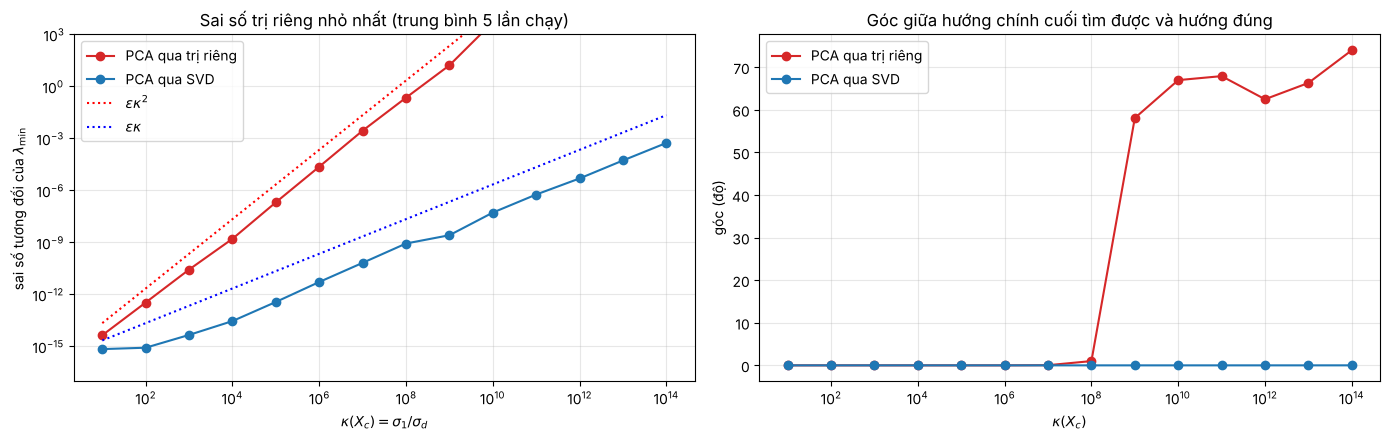
\includegraphics[width=\linewidth]{img/A_c07_0.png}
\end{center}
\textbf{Đọc hình:} đường đỏ (trị riêng) song song với $\varepsilon\kappa^2$, đường xanh (SVD) song song với $\varepsilon\kappa$. Từ $\kappa\approx10^9$ cách trị riêng sai hoàn toàn, hướng chính cuối lệch hàng chục độ; SVD vẫn đúng.

\begin{ask}
\textbf{Vậy khi nào dùng cách trị riêng?} Khi $d$ nhỏ, $n\gg d$ và dữ liệu điều kiện tốt: chỉ phân rã ma trận $d\times d$ nên nhanh hơn. Sklearn và mọi cài đặt về sau trong đề tài dùng SVD.

\textbf{Vì sao $U$ phải trực giao với vector $\mathbf 1$?} Để $X_c$ đã có trung bình 0; nếu không, bước trừ trung bình trong \code{pca\_*} sẽ thay đổi $X_c$ và đáp án ``biết trước'' không còn đúng.
\end{ask}

\subsection{A.2 SVD ngẫu nhiên và PCA tăng dần}
\subsubsection*{SVD ngẫu nhiên (Halko, Martinsson \& Tropp 2011)}
\begin{minted}{python}
def randomized_svd(A, k, p=10, q=2, rng=None):
    rng = np.random.default_rng(rng)
    m, n = A.shape
    Omega = rng.standard_normal((n, k + p))      # (1) ma trận thử Gauss
    Q, _ = np.linalg.qr(A @ Omega)               #     Y = A Omega, trực chuẩn hóa
    for _ in range(q):                           # (2) lặp lũy thừa có trực chuẩn hóa lại
        Z, _ = np.linalg.qr(A.T @ Q)
        Q, _ = np.linalg.qr(A @ Z)
    B = Q.T @ A                                  # (3) ma trận nhỏ (k+p) x n
    Ub, S, Vt = np.linalg.svd(B, full_matrices=False)
    return (Q @ Ub)[:, :k], S[:k], Vt[:k]
\end{minted}
\begin{enumerate}[label=(\arabic*)]
\item $Y=A\Omega$: mỗi cột là tổ hợp ngẫu nhiên các cột của $A$, nên nằm chủ yếu trong không gian cột chính. $p=10$ cột dự phòng (oversampling) để chắc chắn bắt đủ $k$ hướng.
\item Mỗi vòng nhân thêm $AA^\top$ $\Rightarrow$ giá trị kỳ dị thành $\sigma_i^{2q+1}$, tách rõ $\sigma_k$ khỏi $\sigma_{k+1}$ khi phổ giảm chậm. QR sau \emph{mỗi} phép nhân là bắt buộc: không có nó, mọi cột hội tụ về cùng hướng $u_1$ do sai số làm tròn (đúng như B.5).
\item $A\approx QQ^\top A=QB$; SVD ma trận nhỏ $B=\tilde US V^\top$ cho $A\approx(Q\tilde U)SV^\top$.
\end{enumerate}
\textbf{Kết quả} trên ma trận $2000\times500$, $\sigma_i=i^{-1/2}$ (phổ giảm chậm), $k=20$, tỉ số $\|A-\hat A_k\|_2/\sigma_{k+1}$ (bằng 1 là tối ưu theo Eckart–Young):
\begin{center}
\begin{tabular}{lc}
\toprule
\textbf{Phương pháp} & $\|A-\hat A_k\|_2/\sigma_{k+1}$ \\
\midrule
tự cài, $q=0$ & $2{,}05\pm0{,}14$ \\
tự cài, $q=1$ & $1{,}10\pm0{,}06$ \\
tự cài, $q=2$ & $1{,}015\pm0{,}014$ \\
tự cài, $q=3$ & $1{,}002\pm0{,}002$ \\
tự cài, $q=4$ & $1{,}0003\pm0{,}0004$ \\
\code{sklearn} (\code{n\_iter=2}) & $1{,}015\pm0{,}007$ \\
\bottomrule
\end{tabular}
\end{center}

\subsubsection*{PCA tăng dần cho dữ liệu dòng}
Chỉ lưu $n$, $\mu$ và phác thảo $S_kV_k^\top$ ($k\times d$). Với lô mới $X_b$ ($n_b$ mẫu, trung bình $\mu_b$), ma trận tán xạ toàn bộ thỏa
\[\mathcal S_{\text{mới}}=\mathcal S_{\text{cũ}}+X_{b,c}^\top X_{b,c}+\tfrac{n\,n_b}{n+n_b}(\mu-\mu_b)(\mu-\mu_b)^\top,\]
nên chỉ cần SVD của ma trận xếp chồng $M$ ở dòng 9 dưới đây ($M^\top M=\mathcal S_{\text{mới}}$ khi không cắt cụt).
\begin{minted}{python}
def partial_fit(self, Xb):
    nb, mb = Xb.shape[0], Xb.mean(axis=0)
    if self.n == 0:
        M = Xb - mb
        new_mean = mb
    else:
        corr = np.sqrt(self.n * nb / (self.n + nb)) * (self.mean_ - mb)
        M = np.vstack([self.S_[:, None] * self.Vt_, Xb - mb, corr])
        new_mean = (self.n * self.mean_ + nb * mb) / (self.n + nb)
    _, S, Vt = np.linalg.svd(M, full_matrices=False)
    self.S_, self.Vt_ = S[:self.k], Vt[:self.k]
    self.n += nb
    self.mean_ = new_mean
    self.explained_variance_ = self.S_**2 / (self.n - 1)
\end{minted}
\begin{itemize}
\item \code{self.S\_[:, None] * self.Vt\_} $=S_kV_k^\top$: broadcasting nhân hàng $i$ của $V^\top$ với $\sigma_i$.
\item Dòng \code{corr} là hàng hiệu chỉnh do trung bình dịch chuyển — thiếu nó, kết quả sai khi các lô có trung bình khác nhau.
\end{itemize}
\textbf{Kết quả} (5000 mẫu, 50 chiều, lô 100 mẫu): góc chính lớn nhất so với PCA toàn bộ dữ liệu là $(3{,}1\pm1{,}3)\times10^{-12}$ độ khi không cắt cụt ($k=d$, chính xác) và $(6{,}4\pm2{,}2)\times10^{-4}$ độ khi $k=5$ — trùng với \code{sklearn.IncrementalPCA}. Bộ nhớ: 250 số thay vì 250\,000.

\begin{ask}
\textbf{$p$ và $q$ ảnh hưởng thế nào?} $p$ tăng xác suất bắt đủ không gian con (chặn sai số có hệ số $1+\sqrt{k/(p-1)}$); $q$ làm số hạng đuôi bị nâng lũy thừa $1/(2q+1)$ nên quan trọng khi phổ giảm chậm. Chi phí tăng tuyến tính theo $2q+1$.

\textbf{PCA tăng dần dùng ở Phần D thế nào?} Cập nhật mô hình trạng thái bình thường theo thời gian khi tín hiệu rung đến liên tục, không cần lưu toàn bộ dữ liệu.
\end{ask}

\subsection{A.3 PCA hàm nhân và bộ tự mã hóa tuyến tính}
\subsubsection*{PCA hàm nhân}
\begin{minted}{python}
def fit(self, X):
    self.X_ = X
    K = self.kernel(X, X, self.gamma)
    self.col_mean_ = K.mean(axis=0)
    self.all_mean_ = K.mean()
    Kc = K - self.col_mean_[None, :] - self.col_mean_[:, None] + self.all_mean_   # (1) quy tâm
    ell, A = np.linalg.eigh(Kc)                                                 # (2) phân rã
    order = np.argsort(ell)[::-1][:self.k]
    self.ell_, A = ell[order], A[:, order]
    self.alpha_ = A / np.sqrt(self.ell_)            # chuẩn hóa ||v_j|| = 1
    self.train_scores_ = A * np.sqrt(self.ell_)     # = Kc @ alpha

def transform(self, Y):                             # (3) chiếu điểm mới
    Ky = self.kernel(Y, self.X_, self.gamma)
    Kyc = Ky - Ky.mean(axis=1, keepdims=True) - self.col_mean_[None, :] + self.all_mean_
    return Kyc @ self.alpha_
\end{minted}
\begin{itemize}
\item \textbf{Dòng 6} là công thức $\tilde K=K-\mathbf 1_nK-K\mathbf 1_n+\mathbf 1_nK\mathbf 1_n$ viết bằng broadcasting: trừ trung bình cột, trừ trung bình hàng (với $K$ đối xứng hai cái bằng nhau), cộng trung bình toàn bộ. Đây là quy tâm $\phi(x_i)$ trong không gian đặc trưng mà không cần biết $\phi$.
\item \textbf{Dòng 10}: hướng chính $v_j=\sum_i\alpha_{ij}\phi(x_i)$ có $\|v_j\|^2=\alpha_j^\top\tilde K\alpha_j=\ell_j\|\alpha_j\|^2$, nên $\alpha_j=a_j/\sqrt{\ell_j}$ cho $\|v_j\|=1$.
\item \textbf{Dòng 16}: điểm mới phải quy tâm bằng trung bình \emph{của tập huấn luyện} (\code{col\_mean\_}, \code{all\_mean\_}), giống \code{transform} của PCA thường dùng \code{mean\_} cũ.
\item \code{rbf\_kernel} tính $\|x-y\|^2=\|x\|^2+\|y\|^2-2x^\top y$ cho mọi cặp bằng một phép nhân ma trận; \code{np.maximum(sq, 0)} chặn số âm nhỏ do làm tròn.
\end{itemize}
\textbf{Kết quả.} Với nhân tuyến tính $k(x,y)=x^\top y$: tọa độ trùng PCA (sai lệch $7\times10^{-15}$) và $\ell_j/(n-1)=\lambda_j$. Với RBF: trùng \code{sklearn.KernelPCA} (sai lệch $4\times10^{-15}$, cả với điểm mới). Trên dữ liệu hai vòng tròn, độ chính xác tách lớp chỉ bằng thành phần 1:
\begin{center}
\begin{tabular}{lcccccc}
\toprule
& PCA tuyến tính & $\gamma=1$ & $\gamma=2$ & $\gamma=5$ & $\gamma=10$ & $\gamma=15$ \\
\midrule
độ chính xác & 0,497 & 0,497 & 0,510 & \textbf{1,000} & 0,688 & 0,743 \\
\bottomrule
\end{tabular}
\end{center}
\begin{center}
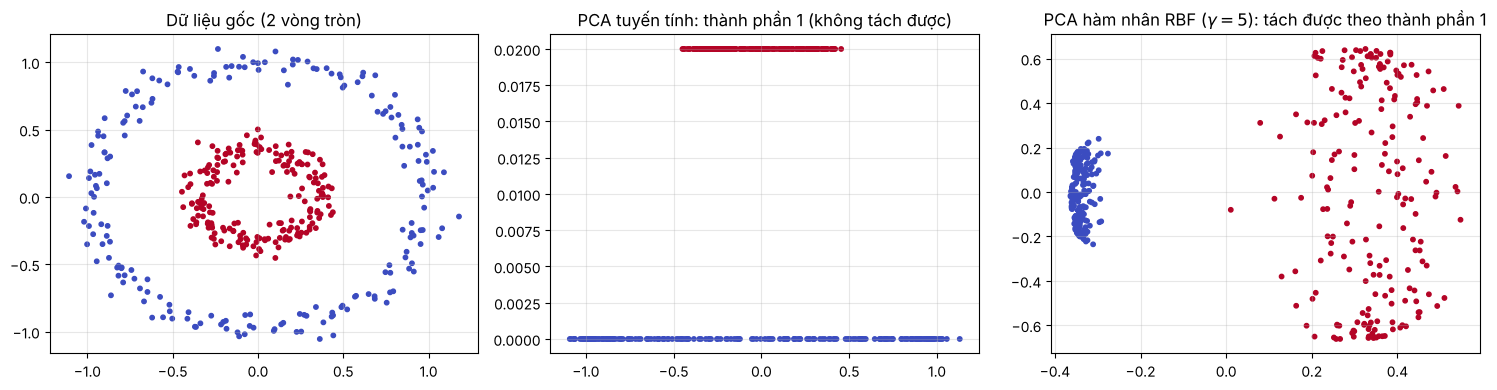
\includegraphics[width=\linewidth]{img/A_c16_0.png}
\end{center}
$\gamma$ quá nhỏ: nhân gần tuyến tính; quá lớn: mỗi điểm chỉ ``thấy'' lân cận rất hẹp. Ở Phần D, $\gamma$ phải chọn trên tập kiểm định.

\subsubsection*{Bộ tự mã hóa tuyến tính huấn luyện bằng hạ gradient}
Mô hình $\hat X=X_cE^\top D^\top$, mất mát $\mathcal L=\frac1n\|X_c-X_cE^\top D^\top\|_F^2$. Đặt $Z=X_cE^\top$, $R=ZD^\top-X_c$. \textbf{Dẫn xuất gradient:} $\mathcal L=\frac1n\operatorname{tr}(R^\top R)$, vi phân $d\mathcal L=\frac2n\operatorname{tr}(R^\top dR)$.
\begin{itemize}
\item Theo $D$: $dR=Z\,dD^\top$ $\Rightarrow$ $d\mathcal L=\frac2n\operatorname{tr}(R^\top Z\,dD^\top)=\frac2n\operatorname{tr}(dD\,Z^\top R)$ $\Rightarrow$ $\nabla_D\mathcal L=\frac2nR^\top Z$.
\item Theo $E$: $dR=X_c\,dE^\top D^\top$ $\Rightarrow$ $d\mathcal L=\frac2n\operatorname{tr}(R^\top X_c\,dE^\top D^\top)=\frac2n\operatorname{tr}(dE\,X_c^\top RD)$ $\Rightarrow$ $\nabla_E\mathcal L=\frac2nD^\top R^\top X_c$.
\end{itemize}
\begin{minted}{python}
def loss_and_grads(self, Xc, E, D):
    n = Xc.shape[0]
    Z = Xc @ E.T                       # n x k
    R = Z @ D.T - Xc                   # phần dư n x d
    loss = (R**2).sum() / n
    gD = 2.0 / n * R.T @ Z             # d x k
    gE = 2.0 / n * D.T @ R.T @ Xc      # k x d
    return loss, gE, gD
\end{minted}
\begin{itemize}
\item \textbf{Kiểm tra gradient} bằng sai phân trung tâm $\frac{\mathcal L(\theta+h)-\mathcal L(\theta-h)}{2h}$ với $h=10^{-6}$: sai số tương đối $6\times10^{-10}$ cho cả $E$ và $D$ $\Rightarrow$ công thức đúng.
\item \textbf{Bước học} $\eta=0{,}4/\lambda_1$ (với $\lambda_1$ tính theo $1/n$): độ cong của $\mathcal L$ tỉ lệ với $\lambda_1$, bước lớn hơn $\sim2/\text{độ cong}$ sẽ phân kỳ.
\item Khởi tạo ngẫu nhiên nhỏ ($0{,}1\times$ Gauss); khởi tạo bằng 0 sẽ làm cả hai gradient bằng 0 mãi mãi.
\end{itemize}
\textbf{Kết quả} (Wine, $k=3$, 3000 vòng, 5 khởi tạo): $\mathcal L/\mathcal L^\star-1\approx2\times10^{-16}$; góc giữa $\operatorname{span}(D)$ và không gian con PCA $\approx7\times10^{-14}$ độ; $\max|DE-V_kV_k^\top|\approx1{,}5\times10^{-15}$; nhưng $\max|D^\top D-I|=0{,}038\pm0{,}014$ — $D$ \emph{không} trực chuẩn. Đúng như mệnh đề B.3: chỉ không gian con và phép chiếu $DE$ là duy nhất.
\begin{center}
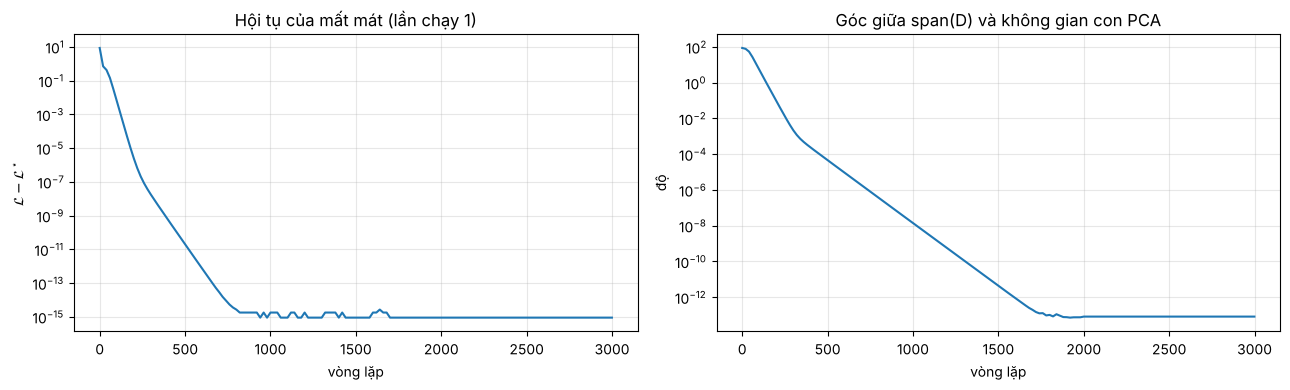
\includegraphics[width=0.95\linewidth]{img/A_c20_0.png}
\end{center}

\begin{ask}
\textbf{Bộ tự mã hóa tuyến tính khác PCA ở đâu?} Cùng không gian con, cùng sai số tái tạo tối ưu, nhưng các cột của $D$ không trực chuẩn và không sắp theo phương sai; PCA cho cơ sở trực chuẩn có thứ tự. Bộ tự mã hóa phi tuyến (thêm hàm kích hoạt) mới vượt được PCA.

\textbf{Vì sao hạ gradient không kẹt ở cực tiểu địa phương?} Baldi \& Hornik (1989): mọi điểm dừng khác của $\mathcal L$ là điểm yên ngựa.
\end{ask}

\subsection{A.4 Thống kê giám sát $T^2$ Hotelling và SPE}
\textbf{Ý tưởng.} PCA học từ dữ liệu \emph{bình thường} chia không gian thành không gian con chính ($k$ chiều, biến thiên hợp lệ) và không gian dư. $T^2=\sum_{i\le k}t_i^2/\lambda_i$ đo độ lệch \emph{trong} không gian con chính (chuẩn hóa theo phương sai từng hướng); $\mathrm{SPE}=\|x-PP^\top x\|^2$ đo phần \emph{ngoài} không gian con — tức mức phá vỡ cấu trúc tương quan.

\begin{minted}{python}
def fit(self, X):
    n, d = X.shape
    self.mean_ = X.mean(axis=0)
    self.std_ = X.std(axis=0, ddof=1)
    self.std_[self.std_ == 0] = 1.0
    Z = (X - self.mean_) / self.std_
    _, S, Vt = np.linalg.svd(Z, full_matrices=False)
    lam = S**2 / (n - 1)
    if self.k is None:
        self.k = int(np.searchsorted(np.cumsum(lam) / lam.sum(), self.var_ratio) + 1)
    k, a = self.k, self.alpha
    self.P_, self.lam_, self.n_ = Vt[:k].T, lam, n
    self.T2_lim_chi2_ = stats.chi2.ppf(1 - a, k)
    self.T2_lim_F_ = k * (n - 1) * (n + 1) / (n * (n - k)) * stats.f.ppf(1 - a, k, n - k)
    res = lam[k:]
    th1, th2, th3 = res.sum(), (res**2).sum(), (res**3).sum()
    h0 = 1 - 2 * th1 * th3 / (3 * th2**2)
    ca = np.sign(h0) * stats.norm.ppf(1 - a)
    self.SPE_lim_JM_ = th1 * (ca * np.sqrt(2 * th2 * h0**2) / th1 + 1 + th2 * h0 * (h0 - 1) / th1**2) ** (1 / h0)
    g, h = th2 / th1, th1**2 / th2
    self.SPE_lim_box_ = g * stats.chi2.ppf(1 - a, h)
\end{minted}
\begin{itemize}
\item \textbf{Dòng 3–6}: chuẩn hóa bằng thống kê \emph{của dữ liệu bình thường} (PCA trên ma trận tương quan — lý do ở C.2). Cột có độ lệch chuẩn 0 được gán 1 để tránh chia cho 0.
\item \textbf{Dòng 9–10}: nếu không cho \code{k}, chọn $k$ nhỏ nhất đạt \code{var\_ratio} phương sai tích lũy; \code{searchsorted} tìm vị trí đầu tiên $\ge$ ngưỡng.
\item \textbf{Dòng 13}: giới hạn $\chi^2_k$ — đúng khi hiệp phương sai đã biết (B.6).
\item \textbf{Dòng 14}: giới hạn $F$ cho quan sát mới khi $\mu$, $\Sigma$ ước lượng từ $n$ mẫu.
\item \textbf{Dòng 15–20}: Jackson–Mudholkar. $\theta_j=\sum_{i>k}\lambda_i^j$ dùng các trị riêng \emph{phần dư}. Chú ý \code{np.sign(h0)}: $c_\alpha$ phải cùng dấu với $h_0$; khi trị riêng phần dư rất chênh lệch thì $h_0<0$ và bỏ dấu này làm giới hạn sai hoàn toàn (lỗi này đã gặp và sửa khi viết notebook: tỉ lệ báo động giả từng lên tới 80\%).
\item \textbf{Dòng 21–22}: xấp xỉ Box $g\chi^2_h$ khớp trung bình $\theta_1$ và phương sai $2\theta_2$ của SPE.
\end{itemize}
\begin{minted}{python}
def scores(self, X):
    Z = (X - self.mean_) / self.std_
    T = Z @ self.P_                                   # tọa độ trên các thành phần chính
    T2 = (T**2 / self.lam_[:self.k]).sum(axis=1)
    E = Z - T @ self.P_.T                             # phần dư ngoài không gian con chính
    SPE = (E**2).sum(axis=1)
    return T2, SPE
\end{minted}
\code{fit\_empirical\_limits(X\_val)} lấy phân vị $1-\alpha$ của $T^2$, SPE trên dữ liệu bình thường kiểm định; \code{predict(..., rule="either")} báo động nếu một trong hai vượt giới hạn.

\textbf{Thí nghiệm.} Quá trình 20 cảm biến từ 3 nhân tố ẩn ($x=Lf+e$, nhiễu $0{,}3$). Huấn luyện 1000 mẫu bình thường, ngưỡng thực nghiệm trên 1000 mẫu khác, kiểm tra 2000 mẫu bình thường và 2 loại lỗi; 5 lần chạy, $\alpha=0{,}01$.
\begin{center}
\begin{tabular}{lc@{\qquad}lc}
\toprule
\multicolumn{2}{c}{\textbf{Tỉ lệ báo động giả (mục tiêu 0,01)}} & \multicolumn{2}{c}{\textbf{Tỉ lệ phát hiện}} \\
\midrule
$T^2$, $\chi^2_k$ & $0{,}0125\pm0{,}0025$ & Lỗi 1 (nhân tố 1 $+5$), $T^2$ & $0{,}969\pm0{,}011$ \\
$T^2$, $F$ & $0{,}0119\pm0{,}0023$ & Lỗi 1, SPE & $0{,}008\pm0{,}003$ \\
$T^2$, thực nghiệm & $0{,}0145\pm0{,}0057$ & Lỗi 2 (cảm biến 5 $+3$), $T^2$ & $0{,}014\pm0{,}006$ \\
SPE, Jackson–Mudholkar & $0{,}0075\pm0{,}0015$ & Lỗi 2, SPE & $0{,}958\pm0{,}057$ \\
SPE, Box & $0{,}0162\pm0{,}0035$ & & \\
SPE, thực nghiệm & $0{,}0115\pm0{,}0014$ & & \\
\bottomrule
\end{tabular}
\end{center}
\begin{center}
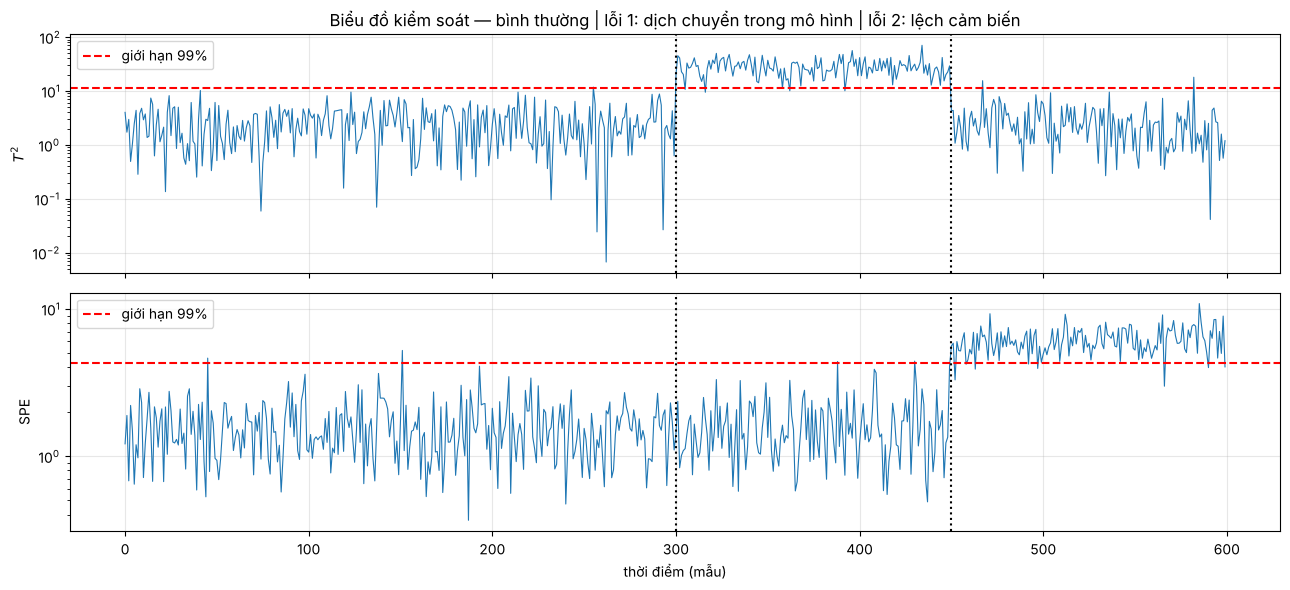
\includegraphics[width=0.95\linewidth]{img/A_c25_0.png}
\end{center}
\textbf{Đọc kết quả:} lỗi 1 làm biến thiên lớn nhưng \emph{đúng cấu trúc tương quan} $\Rightarrow$ chỉ $T^2$ bắt. Lỗi 2 làm một cảm biến lệch khỏi quan hệ với các cảm biến khác $\Rightarrow$ chỉ SPE bắt. Hai thống kê bổ sung cho nhau nên Phần D dùng quy tắc ``either''.

\begin{ask}
\textbf{Vì sao giới hạn $F$ tốt hơn $\chi^2$?} $\chi^2$ giả sử hiệp phương sai biết đúng; khi ước lượng từ mẫu, $T^2$ có đuôi nặng hơn — $F$ tính đến điều này (thấy rõ ở B.6 với $n=30$).

\textbf{Khi nào dùng giới hạn thực nghiệm?} Khi dữ liệu không chuẩn (đặc trưng rung thường lệch phải) — giới hạn lý thuyết khi đó không bảo đảm tỉ lệ báo động giả.
\end{ask}

\subsection{Ô kiểm tra đồng bộ}
Ô cuối Notebook 1 import \code{pca\_core} và so sánh kết quả của 7 thành phần (\code{pca\_eig}, \code{pca\_svd}, \code{randomized\_svd}, \code{StreamingPCA}, \code{KernelPCA\_}, \code{LinearAutoencoder}, \code{PCAMonitor}) với cài đặt trong notebook bằng \code{np.allclose}. Kết quả: cả 7 đều \code{khớp}.

%=====================================================================
\section{Notebook 2 — Phần B: Chứng minh lý thuyết}
%=====================================================================
Mục này chứa toàn văn chứng minh (giống Notebook 2), dạng LaTeX để dùng trực tiếp trong báo cáo. Sau mỗi chứng minh là mô tả ô kiểm chứng số và kết quả.

Mỗi mục gồm: \textbf{phát biểu} (đủ giả thiết) \(\to\) \textbf{chứng minh} \(\to\) \textbf{kiểm chứng số}. Ký hiệu \(\langle\cdot,\cdot\rangle\), \(\|\cdot\|\) là tích vô hướng và chuẩn Euclid; \(\|M\|_F^2=\operatorname{tr}(M^\top M)=\sum_{ij}M_{ij}^2\).

\textbf{Hai sự kiện dùng nhiều lần.}

\begin{itemize}

\item
  \textbf{(F1) Phép chiếu trực giao.} Nếu \(U\in\mathbb R^{d\times k}\) có \(U^\top U=I_k\) thì \(P=UU^\top\) thỏa \(P^\top=P\), \(P^2=P\); với mọi \(x\): \(x-Px\perp Px\) (vì \(U^\top(x-UU^\top x)=0\)), nên \(\|x\|^2=\|Px\|^2+\|x-Px\|^2\) (Pythagoras) và \(\|Px\|^2=\|U^\top x\|^2\le\|x\|^2\).
\item
  \textbf{(F2) Vết bất biến hoán vị vòng:} \(\operatorname{tr}(ABC)=\operatorname{tr}(CAB)\).
\end{itemize}


\subsection{B.1 Cực đại phương sai $\Leftrightarrow$ cực tiểu sai số tái tạo; định lý Ky Fan}
\textbf{Phát biểu.} Cho \(\Sigma\in\mathbb R^{d\times d}\) đối xứng với trị riêng \(\lambda_1\ge\dots\ge\lambda_d\) và vector riêng trực chuẩn \(v_1,\dots,v_d\); \(1\le k\le d\), \(V_k=[v_1,\dots,v_k]\).

\begin{enumerate}
\def\labelenumi{\arabic{enumi}.}

\item
  \emph{(Ky Fan)} \(\displaystyle\max_{U\in\mathbb R^{d\times k},\,U^\top U=I_k}\operatorname{tr}(U^\top\Sigma U)=\sum_{i=1}^k\lambda_i\), đạt tại \(U=V_k\). Nếu thêm \(\lambda_k>\lambda_{k+1}\) thì giá trị lớn nhất đạt \textbf{khi và chỉ khi} \(\operatorname{span}(U)=\operatorname{span}(V_k)\). Trường hợp \(k=1\): \(\max_{\|u\|=1}u^\top\Sigma u=\lambda_1\) (thương Rayleigh).
\item
  \emph{(Tương đương)} Với dữ liệu đã quy tâm \(x_1,\dots,x_n\) và \(\Sigma=\frac1{n-1}\sum_i x_ix_i^\top\), mọi \(U\) có \(U^\top U=I_k\) thỏa \[\underbrace{\frac1{n-1}\sum_{i=1}^n\|x_i-UU^\top x_i\|^2}_{\text{sai số tái tạo}}=\operatorname{tr}\Sigma-\underbrace{\operatorname{tr}(U^\top\Sigma U)}_{\text{phương sai của dữ liệu chiếu}} .\] Do \(\operatorname{tr}\Sigma\) không phụ thuộc \(U\), \textbf{cực đại phương sai chiếu và cực tiểu sai số tái tạo có cùng tập nghiệm}.
\end{enumerate}

\textbf{Chứng minh (2).} Theo (F1), \(\|x_i\|^2=\|U^\top x_i\|^2+\|x_i-UU^\top x_i\|^2\). Lấy tổng và chia \(n-1\): \(\frac1{n-1}\sum_i\|x_i\|^2=\operatorname{tr}\big(\frac1{n-1}\sum_ix_ix_i^\top\big)=\operatorname{tr}\Sigma\) và \(\frac1{n-1}\sum_i\|U^\top x_i\|^2=\operatorname{tr}\big(U^\top\Sigma U\big)\) (dùng (F2)). Vì \(\sum_iU^\top x_i=U^\top\sum_ix_i=0\), đại lượng này đúng là tổng phương sai của các tọa độ chiếu \(U^\top x_i\). \(\square\)

\textbf{Chứng minh (1).} Viết \(\Sigma=V\Lambda V^\top\). Theo (F2), \(\operatorname{tr}(U^\top\Sigma U)=\operatorname{tr}(\Lambda\,V^\top UU^\top V)=\sum_{i=1}^d\lambda_iw_i\), với \(w_i=v_i^\top UU^\top v_i=\|U^\top v_i\|^2\). Các trọng số thỏa:

\begin{itemize}

\item
  \(0\le w_i\le1\) --- theo (F1), \(\|U^\top v_i\|^2\le\|v_i\|^2=1\);
\item
  \(\sum_iw_i=\operatorname{tr}(V^\top UU^\top V)=\operatorname{tr}(U^\top VV^\top U)=\operatorname{tr}(U^\top U)=k\).
\end{itemize}

Khi đó \[\sum_i\lambda_iw_i-\sum_{i\le k}\lambda_i=\sum_{i\le k}\lambda_i(w_i-1)+\sum_{i>k}\lambda_iw_i\le\lambda_k\sum_{i\le k}(w_i-1)+\lambda_k\sum_{i>k}w_i=\lambda_k\Big(\sum_iw_i-k\Big)=0,\] trong đó bất đẳng thức dùng: với \(i\le k\), \(w_i-1\le0\) và \(\lambda_i\ge\lambda_k\); với \(i>k\), \(w_i\ge0\) và \(\lambda_i\le\lambda_k\). Tại \(U=V_k\): \(w_i=1\) (\(i\le k\)), \(w_i=0\) (\(i>k\)), nên đạt dấu bằng.

\emph{Duy nhất.} Phần chênh lệch đúng bằng \(-\sum_{i\le k}(\lambda_i-\lambda_k)(1-w_i)-\sum_{i>k}(\lambda_k-\lambda_i)w_i\), tổng các số hạng không dương. Dấu bằng buộc \((\lambda_k-\lambda_i)w_i=0\) với mọi \(i>k\); nếu \(\lambda_k>\lambda_{k+1}\ge\lambda_i\) thì \(w_i=\|U^\top v_i\|^2=0\), tức \(\operatorname{span}(U)\perp v_{k+1},\dots,v_d\), nên \(\operatorname{span}(U)\subseteq\operatorname{span}(V_k)\); hai không gian cùng \(k\) chiều nên bằng nhau. Chiều ngược lại: nếu \(\operatorname{span}(U)=\operatorname{span}(V_k)\) thì \(U=V_kG\) với \(G\) trực giao, \(\operatorname{tr}(U^\top\Sigma U)=\operatorname{tr}(G^\top\Lambda_kG)=\sum_{i\le k}\lambda_i\). \(\blacksquare\)

\emph{Ghi chú:} chứng minh không cần \(\Sigma\) nửa xác định dương --- điều này được dùng lại ở B.2 cho \(AA^\top\).

\paragraph{Kiểm chứng số.} $\Sigma$ ngẫu nhiên $30\times30$, $k=5$: trên 5000 ma trận $U$ trực chuẩn ngẫu nhiên, $\max\operatorname{tr}(U^\top\Sigma U)/\sum_{i\le5}\lambda_i=0{,}495<1$; tại $U=V_k$ và $U=V_kG$ ($G$ trực giao) tỉ số đúng bằng 1. Trên Wine: sai số tái tạo $=8{,}0995654759=\operatorname{tr}\Sigma-\operatorname{tr}(U^\top\Sigma U)$.
\begin{ask}
\textbf{Ở đâu dùng $\lambda_i\ge\lambda_k$ và $w_i\le1$?} Trong bất đẳng thức chính: hai điều kiện này làm mọi số hạng chênh lệch không dương.
\textbf{Vì sao cần $\lambda_k>\lambda_{k+1}$ cho tính duy nhất?} Nếu bằng nhau, có thể xoay trong không gian riêng chung mà tổng không đổi.
\end{ask}

\subsection{B.2 Định lý Eckart–Young–Mirsky}
\textbf{Phát biểu.} Cho \(A\in\mathbb R^{m\times n}\) có SVD \(A=\sum_{i=1}^{r}\sigma_iu_iv_i^\top\) (\(\sigma_1\ge\dots\ge\sigma_r>0\), \(r=\operatorname{rank}A\), quy ước \(\sigma_i=0\) khi \(i>r\)), \(1\le k\le\min(m,n)\) và \(A_k=\sum_{i=1}^k\sigma_iu_iv_i^\top\). Khi đó \[\min_{\operatorname{rank}(B)\le k}\|A-B\|_F^2=\sum_{i>k}\sigma_i^2,\] đạt tại \(B=A_k\). Nếu \(\sigma_k>\sigma_{k+1}\) thì \(A_k\) là nghiệm \textbf{duy nhất}.

\textbf{Chứng minh.}

\emph{Bước 1 --- chặn dưới theo một không gian con.} Cho \(B\) với \(\operatorname{rank}B\le k\). Lấy một cơ sở trực chuẩn của \(\operatorname{col}(B)\) và bổ sung cho đủ \(k\) vector trực chuẩn (được vì \(k\le m\)), ghép thành \(Q\in\mathbb R^{m\times k}\), \(Q^\top Q=I_k\), \(\operatorname{col}(B)\subseteq\operatorname{col}(Q)\). Với cột thứ \(j\): \(a_j-b_j=(I-QQ^\top)a_j+(QQ^\top a_j-b_j)\); số hạng đầu vuông góc với \(\operatorname{col}(Q)\), số hạng sau thuộc \(\operatorname{col}(Q)\). Theo Pythagoras, \[\|a_j-b_j\|^2=\|(I-QQ^\top)a_j\|^2+\|QQ^\top a_j-b_j\|^2\ \ge\ \|(I-QQ^\top)a_j\|^2 .\] Cộng theo \(j\): \(\|A-B\|_F^2\ge\|(I-QQ^\top)A\|_F^2\), dấu bằng khi và chỉ khi \(B=QQ^\top A\).

\emph{Bước 2 --- tính chặn dưới.} Theo (F1) áp dụng cho từng cột, \(\|(I-QQ^\top)A\|_F^2=\|A\|_F^2-\|Q^\top A\|_F^2=\|A\|_F^2-\operatorname{tr}(Q^\top AA^\top Q)\). Ngoài ra \(\|A\|_F^2=\operatorname{tr}(A^\top A)=\sum_i\sigma_i^2\).

\emph{Bước 3 --- dùng Ky Fan.} \(AA^\top\) đối xứng, có trị riêng \(\sigma_1^2\ge\sigma_2^2\ge\dots\) (cùng các số 0) với vector riêng \(u_i\). Theo B.1, \(\operatorname{tr}(Q^\top AA^\top Q)\le\sum_{i\le k}\sigma_i^2\). Vậy \[\|A-B\|_F^2\ \ge\ \sum_i\sigma_i^2-\sum_{i\le k}\sigma_i^2=\sum_{i>k}\sigma_i^2 .\]

\emph{Bước 4 --- đạt được.} \(A-A_k=\sum_{i>k}\sigma_iu_iv_i^\top\), và do \(\{u_i\}\), \(\{v_i\}\) trực chuẩn, \(\|A-A_k\|_F^2=\operatorname{tr}\big(\sum_{i>k}\sigma_i^2v_iv_i^\top\big)=\sum_{i>k}\sigma_i^2\).

\emph{Bước 5 --- duy nhất.} Nếu \(\|A-B\|_F^2=\sum_{i>k}\sigma_i^2\) thì mọi bất đẳng thức trên là đẳng thức: (i) theo phần duy nhất của B.1 (với \(\sigma_k^2>\sigma_{k+1}^2\)), \(\operatorname{col}(Q)=\operatorname{span}(u_1,\dots,u_k)\), tức \(QQ^\top=U_kU_k^\top\); (ii) \(B=QQ^\top A=U_kU_k^\top A=A_k\). \(\blacksquare\)

\emph{Hệ quả cho PCA:} với \(A=X_c\), giữ \(k\) thành phần chính đầu là xấp xỉ hạng \(k\) tối ưu của dữ liệu; sai số tái tạo bằng \((n-1)\sum_{i>k}\lambda_i\).

\paragraph{Kiểm chứng số.} $A$ cỡ $60\times40$, $k=5$: $\|A-A_k\|_F^2=\sum_{i>5}\sigma_i^2=4238{,}24680651$; ma trận hạng 5 ngẫu nhiên tốt nhất trong 2000 lần thử cho $15062{,}9$; bình phương tối thiểu luân phiên (cực tiểu hóa $\|A-PQ\|_F$ theo $P$, $Q$ từ 5 khởi tạo) hội tụ về đúng cận dưới, tỉ số $1{,}0000000000$ — không lần nào thấp hơn.
\begin{ask}
\textbf{Định lý có đúng cho chuẩn phổ không?} Có: $\min_{\operatorname{rank}B\le k}\|A-B\|_2=\sigma_{k+1}$ (Mirsky, mọi chuẩn bất biến unita), nhưng nghiệm không duy nhất.
\end{ask}

\subsection{B.3 Bộ tự mã hóa tuyến tính}
\textbf{Phát biểu.} Cho \(X_c\in\mathbb R^{n\times d}\) có SVD \(X_c=U\,\mathrm{diag}(\sigma)V^\top\), \textbf{hạng đầy đủ theo cột} (\(\operatorname{rank}X_c=d\le n\)), và \(\sigma_k>\sigma_{k+1}\). Xét bộ tự mã hóa tuyến tính với bộ mã hóa \(E\in\mathbb R^{k\times d}\), bộ giải mã \(D\in\mathbb R^{d\times k}\), ánh xạ tái tạo \(x\mapsto DEx\), và mất mát \[\mathcal L(E,D)=\|X_c-X_cE^\top D^\top\|_F^2=\sum_{i=1}^n\|x_i-DEx_i\|^2 .\] Khi đó \(\min_{E,D}\mathcal L=\sum_{i>k}\sigma_i^2\), và \((E,D)\) là cực tiểu toàn cục \textbf{khi và chỉ khi} \(DE=V_kV_k^\top\) --- phép chiếu trực giao lên không gian con chính. Hệ quả: \(\operatorname{span}(D)=\operatorname{span}(V_k)\).

\textbf{Chứng minh.} \emph{Chặn dưới.} \(\operatorname{rank}(X_cE^\top D^\top)\le\operatorname{rank}(D^\top)\le k\), nên theo B.2, \(\mathcal L(E,D)\ge\sum_{i>k}\sigma_i^2\) với mọi \((E,D)\).

\emph{Đạt được.} Với \(E=V_k^\top\), \(D=V_k\): \(X_cV_kV_k^\top=\sum_{i\le k}\sigma_iu_iv_i^\top=A_k\) (vì \(X_cv_i=\sigma_iu_i\)), nên \(\mathcal L=\sum_{i>k}\sigma_i^2\).

\emph{Điều kiện cần.} Giả sử \(\mathcal L(E,D)=\sum_{i>k}\sigma_i^2\). Theo phần duy nhất của B.2 (dùng \(\sigma_k>\sigma_{k+1}\)), \(X_cE^\top D^\top=A_k=X_cV_kV_k^\top\), tức \(X_c\big(E^\top D^\top-V_kV_k^\top\big)=0\). Vì \(X_c\) hạng đầy đủ theo cột, \(X_cM=0\Rightarrow M=0\), nên \(E^\top D^\top=V_kV_k^\top\); chuyển vị: \(DE=V_kV_k^\top\). Ma trận này đối xứng và lũy đẳng, ảnh là \(\operatorname{span}(V_k)\): đó là phép chiếu trực giao lên không gian con chính.

\emph{Điều kiện đủ.} Nếu \(DE=V_kV_k^\top\) thì \(X_cE^\top D^\top=X_c(DE)^\top=X_cV_kV_k^\top=A_k\), đạt cực tiểu.

\emph{Hệ quả.} \(\operatorname{span}(V_k)=\operatorname{range}(DE)\subseteq\operatorname{range}(D)\), mà \(\dim\operatorname{range}(D)\le k\), nên \(\operatorname{span}(D)=\operatorname{span}(V_k)\). \(\blacksquare\)

\emph{Nhận xét.} (i) \(D\), \(E\) không duy nhất: với mọi \(G\in GL_k\), cặp \((G^{-1}V_k^\top,\ V_kG)\) cũng tối ưu; vì vậy bộ tự mã hóa \textbf{tìm đúng không gian con PCA nhưng không nhất thiết tìm ra các hướng chính riêng lẻ} (cơ sở trực chuẩn, sắp theo phương sai). (ii) Baldi \& Hornik (1989) chứng minh thêm rằng mọi điểm dừng khác của \(\mathcal L\) là điểm yên ngựa (không có cực tiểu địa phương xấu) --- giải thích vì sao hạ gradient ở A.3 luôn hội tụ về nghiệm toàn cục.

\paragraph{Kiểm chứng số.} Với $G$ khả nghịch ngẫu nhiên, $(G^{-1}V_k^\top,\ V_kG)$ cho $\mathcal L=770{,}1454157678=\sum_{i>3}\sigma_i^2$; $DE$ đối xứng và lũy đẳng nhưng $D^\top D\neq I$. Huấn luyện lại bằng hạ gradient (5 khởi tạo): $\mathcal L/\mathcal L^\star-1=4\times10^{-16}$, $\max|DE-V_kV_k^\top|=1{,}5\times10^{-15}$.

\subsection{B.4 Bổ đề Johnson–Lindenstrauss}
\textbf{Phát biểu.} Cho \(0<\varepsilon<1\), \(n\ge2\) điểm \(x_1,\dots,x_n\in\mathbb R^d\), số nguyên \(k\ge\dfrac{4\ln n}{\varepsilon^2/2-\varepsilon^3/3}\), ma trận \(R\in\mathbb R^{k\times d}\) có các phần tử \(R_{ij}\sim\mathcal N(0,1)\) độc lập, và \(f(x)=Rx/\sqrt k\). Khi đó với xác suất ít nhất \(1/n\), mọi cặp \(u,v\) trong \(n\) điểm thỏa \[(1-\varepsilon)\|u-v\|^2\le\|f(u)-f(v)\|^2\le(1+\varepsilon)\|u-v\|^2 .\]

\textbf{Chứng minh.} \emph{Bước 1 --- phân phối của một cặp.} Cố định \(u\ne v\), đặt \(z=u-v\). Do \(f\) tuyến tính, \(f(u)-f(v)=Rz/\sqrt k\). Hàng thứ \(j\) của \(R\) là \(r_j\sim\mathcal N(0,I_d)\) nên \(r_j^\top z\sim\mathcal N(0,\|z\|^2)\), và các \(r_j^\top z\) độc lập theo \(j\). Vậy \[Y:=\frac{\|Rz\|^2}{\|z\|^2}=\sum_{j=1}^k\Big(\frac{r_j^\top z}{\|z\|}\Big)^2\sim\chi^2_k,\qquad \frac{\|f(u)-f(v)\|^2}{\|u-v\|^2}=\frac Yk .\] (Nếu \(u=v\) thì bất đẳng thức hiển nhiên đúng.)

\emph{Bước 2 --- hàm sinh mômen.} Với \(g\sim\mathcal N(0,1)\) và \(t<1/2\): \(\mathbb E e^{tg^2}=\int\frac{1}{\sqrt{2\pi}}e^{-(1-2t)g^2/2}dg=(1-2t)^{-1/2}\). Do độc lập, \(\mathbb Ee^{tY}=(1-2t)^{-k/2}\).

\emph{Bước 3 --- đuôi trên.} Với \(0<t<1/2\), theo bất đẳng thức Markov cho \(e^{tY}\): \(\Pr[Y\ge(1+\varepsilon)k]\le e^{-t(1+\varepsilon)k}(1-2t)^{-k/2}\). Chọn \(t=\frac{\varepsilon}{2(1+\varepsilon)}\) (khi đó \(1-2t=\frac1{1+\varepsilon}\)): \[\Pr[Y\ge(1+\varepsilon)k]\le\big((1+\varepsilon)e^{-\varepsilon}\big)^{k/2}=\exp\Big(\tfrac k2\big(\ln(1+\varepsilon)-\varepsilon\big)\Big)\le\exp\Big(-\tfrac k2\big(\tfrac{\varepsilon^2}2-\tfrac{\varepsilon^3}3\big)\Big),\] dùng \(\ln(1+\varepsilon)\le\varepsilon-\frac{\varepsilon^2}2+\frac{\varepsilon^3}3\) với \(\varepsilon\ge0\) (hàm \(h(\varepsilon)=\varepsilon-\frac{\varepsilon^2}2+\frac{\varepsilon^3}3-\ln(1+\varepsilon)\) có \(h(0)=0\), \(h'(\varepsilon)=\frac{\varepsilon^3}{1+\varepsilon}\ge0\)).

\emph{Bước 4 --- đuôi dưới.} Với \(t>0\): \(\Pr[Y\le(1-\varepsilon)k]=\Pr[e^{-tY}\ge e^{-t(1-\varepsilon)k}]\le e^{t(1-\varepsilon)k}(1+2t)^{-k/2}\). Chọn \(t=\frac{\varepsilon}{2(1-\varepsilon)}\) (\(1+2t=\frac1{1-\varepsilon}\)): \[\Pr[Y\le(1-\varepsilon)k]\le\big((1-\varepsilon)e^{\varepsilon}\big)^{k/2}\le\exp\Big(-\tfrac{k\varepsilon^2}4\Big)\le\exp\Big(-\tfrac k2\big(\tfrac{\varepsilon^2}2-\tfrac{\varepsilon^3}3\big)\Big),\] dùng \(\ln(1-\varepsilon)\le-\varepsilon-\frac{\varepsilon^2}2\) (khai triển Taylor, mọi số hạng âm) và \(\varepsilon^3/3\ge0\).

\emph{Bước 5 --- chặn hợp.} Với \(k\ge\frac{4\ln n}{\varepsilon^2/2-\varepsilon^3/3}\) (mẫu số dương vì \(\varepsilon<1\)): \(\frac k2(\frac{\varepsilon^2}2-\frac{\varepsilon^3}3)\ge2\ln n\), nên mỗi đuôi \(\le n^{-2}\) và một cặp bị méo với xác suất \(\le 2/n^2\). Có \(\binom n2\) cặp, theo chặn hợp: \[\Pr[\exists\text{ cặp bị méo}]\le\binom n2\frac2{n^2}=\frac{n-1}n=1-\frac1n .\] Vậy xác suất mọi cặp đều thỏa ít nhất \(1/n\). \(\blacksquare\)

\emph{Nhận xét.} Xác suất \(1/n\) có vẻ nhỏ, nhưng lặp lại \(O(n)\) phép chiếu độc lập là gần như chắc chắn thành công; trên thực tế chặn này rất bảo thủ (xem C.3). Điểm mấu chốt: \(k\) \textbf{chỉ phụ thuộc \(\ln n\) và \(\varepsilon\), không phụ thuộc \(d\)}.

\paragraph{Kiểm chứng số.} $d=200$, $k=40$, 20\,000 ma trận $R$: kiểm định Kolmogorov–Smirnov cho $Y\sim\chi^2_{40}$ có $p=0{,}85$ (không bác bỏ). Đuôi thực nghiệm luôn dưới chặn Chernoff: với $\varepsilon=0{,}3$, $\Pr[Y\ge1{,}3k]=0{,}095$, $\Pr[Y\le0{,}7k]=0{,}076$, chặn $0{,}487$; với $\varepsilon=0{,}5$: $0{,}022$, $0{,}003$, chặn $0{,}189$. Kiểm chứng đầy đủ với $n=1000$ ở C.3.
\begin{ask}
\textbf{Vì sao $k$ không phụ thuộc $d$?} Phân phối của $\|Rz\|^2/\|z\|^2$ là $\chi^2_k$ với \emph{mọi} $z$, không phụ thuộc số chiều $d$ của $z$.
\textbf{Bất đẳng thức nào được dùng?} Markov cho $e^{tY}$ (kỹ thuật Chernoff) và chặn hợp.
\end{ask}

\subsection{B.5 Lặp lũy thừa}
\textbf{Phát biểu.} Cho \(A\in\mathbb R^{d\times d}\) đối xứng, trị riêng \(|\lambda_1|>|\lambda_2|\ge\dots\ge|\lambda_d|\) với vector riêng trực chuẩn \(u_1,\dots,u_d\), và \(v_0\) có \(u_1^\top v_0\neq0\). Lặp \(v_{t+1}=Av_t/\|Av_t\|\). Định nghĩa \(\tan\angle(v,u_1)=\dfrac{\|v-(u_1^\top v)u_1\|}{|u_1^\top v|}\). Khi đó \[\tan\angle(v_t,u_1)\le\Big|\frac{\lambda_2}{\lambda_1}\Big|^t\tan\angle(v_0,u_1).\]

\textbf{Chứng minh.} \emph{Bước 1 --- dạng đóng.} Bằng quy nạp, \(v_t=A^tv_0/\|A^tv_0\|\): đúng với \(t=0\); nếu đúng với \(t\) thì \(Av_t=A^{t+1}v_0/\|A^tv_0\|\), chuẩn hóa ra \(A^{t+1}v_0/\|A^{t+1}v_0\|\). (Mẫu số khác 0 --- xem bước 2.)

\emph{Bước 2 --- khai triển theo cơ sở riêng.} Vì \(A\) đối xứng, \(\{u_i\}\) là cơ sở trực chuẩn: \(v_0=\sum_ic_iu_i\) với \(c_i=u_i^\top v_0\), \(c_1\ne0\). Khi đó \(A^tv_0=\sum_ic_i\lambda_i^tu_i\); thành phần theo \(u_1\) là \(c_1\lambda_1^t\ne0\) (do \(|\lambda_1|>|\lambda_2|\ge0\) nên \(\lambda_1\ne0\)), nên \(A^tv_0\ne0\).

\emph{Bước 3 --- góc.} Góc không đổi khi nhân vector với số dương, nên \[\tan\angle(v_t,u_1)=\frac{\big\|\sum_{i\ge2}c_i\lambda_i^tu_i\big\|}{|c_1\lambda_1^t|}=\frac{\big(\sum_{i\ge2}c_i^2\lambda_i^{2t}\big)^{1/2}}{|c_1||\lambda_1|^t}\le\frac{|\lambda_2|^t\big(\sum_{i\ge2}c_i^2\big)^{1/2}}{|c_1||\lambda_1|^t}=\Big|\frac{\lambda_2}{\lambda_1}\Big|^t\tan\angle(v_0,u_1),\] dùng \(|\lambda_i|\le|\lambda_2|\) với \(i\ge2\) và tính trực chuẩn (Pythagoras). \(\blacksquare\)

\emph{Hệ quả cho A.2/C.4:} tốc độ hội tụ hình học với tỉ số \(|\lambda_2/\lambda_1|\); với SVD (lặp trên \(A^\top A\)) tỉ số là \((\sigma_2/\sigma_1)^2\), và với lặp khối \(k\) vector là \((\sigma_{k+1}/\sigma_k)^2\) --- rất chậm khi phổ suy giảm chậm.

\paragraph{Kiểm chứng số.} Ma trận đối xứng $200\times200$ với $\lambda_1=1$, $\lambda_2=-0{,}9$, các trị riêng còn lại trong $[-0{,}85;0{,}85]$: $\tan\angle(v_t,u_1)$ luôn nằm dưới chặn $0{,}9^t\tan\angle(v_0,u_1)$ trong 120 vòng (danh sách vi phạm rỗng).
\begin{center}
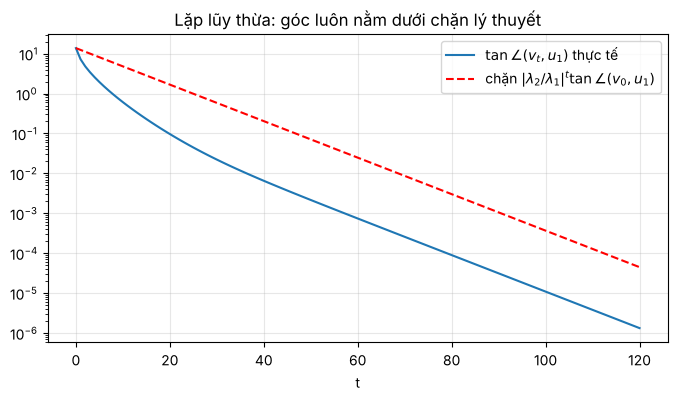
\includegraphics[width=0.6\linewidth]{img/B_c11_0.png}
\end{center}

\subsection{B.6 Phân phối của $T^2$}
\textbf{Phát biểu.} Cho \(x\sim\mathcal N(\mu,\Sigma)\) với \(\mu\), \(\Sigma\) đã biết; \(\Sigma=\sum_i\lambda_iv_iv_i^\top\) (\(\lambda_1\ge\dots\ge\lambda_d\), \(v_i\) trực chuẩn) và \(\lambda_k>0\). Đặt \(t_i=v_i^\top(x-\mu)\) là tọa độ chiếu lên thành phần chính thứ \(i\). Khi đó \[T^2=\sum_{i=1}^k\frac{t_i^2}{\lambda_i}\sim\chi^2_k .\]

\textbf{Chứng minh.} Đặt \(t=V_k^\top(x-\mu)\in\mathbb R^k\). Là ảnh tuyến tính của vector Gauss, \(t\) có phân phối Gauss với trung bình \(V_k^\top\mathbb E(x-\mu)=0\) và hiệp phương sai \(V_k^\top\Sigma V_k=\Lambda_k=\operatorname{diag}(\lambda_1,\dots,\lambda_k)\) (do \(\Sigma v_i=\lambda_iv_i\) và \(v_i\) trực chuẩn). Đặt \(z_i=t_i/\sqrt{\lambda_i}\) (được vì \(\lambda_i\ge\lambda_k>0\)): \(z=\Lambda_k^{-1/2}t\sim\mathcal N(0,I_k)\). Với vector Gauss, không tương quan tương đương độc lập, nên \(z_1,\dots,z_k\) i.i.d. \(\mathcal N(0,1)\). Theo định nghĩa phân phối chi bình phương, \(T^2=\sum_{i\le k}z_i^2\sim\chi^2_k\). \(\blacksquare\)

\emph{Hệ quả.}

\begin{itemize}

\item
  Giới hạn kiểm soát \(T^2_\alpha=\chi^2_{k,1-\alpha}\) cho đúng tỉ lệ báo động giả \(\alpha\).
\item
  Cùng lập luận: \(\mathrm{SPE}=\sum_{i>k}t_i^2=\sum_{i>k}\lambda_iz_i^2\) là \textbf{tổng có trọng số của các \(\chi^2_1\)} --- không có dạng đóng đơn giản, nên cần các xấp xỉ Jackson--Mudholkar hay Box (\(g\chi^2_h\), khớp hai mômen đầu: \(\mathbb E=\theta_1\), \(\operatorname{Var}=2\theta_2\)) dùng ở A.4.
\item
  Khi \(\mu\), \(\Sigma\) \textbf{ước lượng} từ \(n\) mẫu, \(T^2\) của quan sát mới tuân theo \(\frac{k(n-1)(n+1)}{n(n-k)}F_{k,n-k}\) (không chứng minh ở đây); với \(n\) nhỏ, dùng \(\chi^2_k\) sẽ làm tăng báo động giả --- kiểm chứng bên dưới.
\end{itemize}

\paragraph{Kiểm chứng số.} 200\,000 mẫu từ $\mathcal N(\mu,\Sigma)$, $d=10$, $k=3$: Kolmogorov–Smirnov cho $T^2\sim\chi^2_3$ có $p=0{,}68$; $\Pr[T^2>\chi^2_{3;0,99}]=0{,}0100$. Khi ước lượng $\Sigma$ từ chỉ $n=30$ mẫu: tỉ lệ báo động giả với giới hạn $\chi^2$ là $0{,}017\pm0{,}008$ (vượt mục tiêu), với giới hạn $F$ là $0{,}004\pm0{,}003$.
\begin{center}
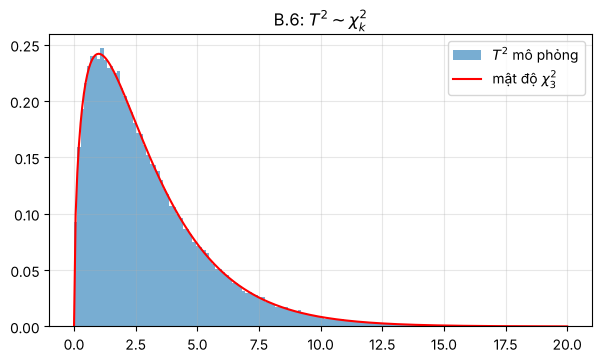
\includegraphics[width=0.55\linewidth]{img/B_c13_0.png}
\end{center}

%=====================================================================
\section{Notebook 3 — Phần C: Bài tập}
%=====================================================================
\subsection{C.1 Tính tay PCA cho bốn điểm}
\textbf{Bước 1 --- trung bình.} \(\mu=\frac14\big(3+1-3-1,\ 1+3-1-3\big)=(0,0)\): dữ liệu đã quy tâm, \(X_c=X=\begin{bmatrix}3&1\\1&3\\-3&-1\\-1&-3\end{bmatrix}\).

\textbf{Bước 2 --- ma trận tán xạ và hiệp phương sai.} \(X^\top X=\begin{bmatrix}9+1+9+1 & 3+3+3+3\\ 3+3+3+3 & 1+9+1+9\end{bmatrix}=\begin{bmatrix}20&12\\12&20\end{bmatrix}\), nên \(\Sigma=\frac1{n-1}X^\top X=\frac13\begin{bmatrix}20&12\\12&20\end{bmatrix}=\begin{bmatrix}20/3&4\\4&20/3\end{bmatrix}\). (Nếu dùng ước lượng hợp lý cực đại \(\frac1n X^\top X=\begin{bmatrix}5&3\\3&5\end{bmatrix}\) thì mọi trị riêng chia cho 4 thay vì 3; hướng chính và tỉ lệ phương sai không đổi.)

\textbf{Bước 3 --- trị riêng, vector riêng.} \(\det\begin{bmatrix}20/3-\lambda&4\\4&20/3-\lambda\end{bmatrix}=(20/3-\lambda)^2-16=0\Rightarrow\lambda=20/3\pm4\): \[\lambda_1=\tfrac{32}3\approx10.667,\quad v_1=\tfrac1{\sqrt2}(1,1);\qquad \lambda_2=\tfrac83\approx2.667,\quad v_2=\tfrac1{\sqrt2}(1,-1).\] (Kiểm tra: \(\Sigma v_1=\frac1{\sqrt2}(20/3+4,\ 4+20/3)=\frac{32}3v_1\).)

\textbf{Bước 4 --- tỉ lệ phương sai giải thích.} \(\dfrac{\lambda_1}{\lambda_1+\lambda_2}=\dfrac{32/3}{40/3}=0.8\), \(\dfrac{\lambda_2}{\lambda_1+\lambda_2}=0.2\).

\textbf{Bước 5 --- sai số tái tạo khi giữ 1 thành phần.} Tọa độ trên \(v_2\): \(\frac{3-1}{\sqrt2}=\sqrt2\), \(\frac{1-3}{\sqrt2}=-\sqrt2\), \(\frac{-3+1}{\sqrt2}=-\sqrt2\), \(\frac{-1+3}{\sqrt2}=\sqrt2\). Phần bị bỏ của mỗi điểm có độ dài bình phương \(2\), nên \[\sum_i\|x_i-v_1v_1^\top x_i\|^2=4\times2=8 .\] Các điểm tái tạo: \((2,2),(2,2),(-2,-2),(-2,-2)\).

\textbf{Bước 6 --- kiểm chứng với B.2.} Giá trị kỳ dị của \(X\): \(\sigma_i^2=(n-1)\lambda_i\), tức \(\sigma_1^2=32\), \(\sigma_2^2=8\) (\(\sigma_1=4\sqrt2\), \(\sigma_2=2\sqrt2\)). Eckart--Young: \(\min_{\operatorname{rank}B\le1}\|X-B\|_F^2=\sigma_2^2=8\) --- \textbf{khớp với bước 5}. Theo B.1: sai số tái tạo chia \(n-1\) là \(8/3=\lambda_2=\operatorname{tr}\Sigma-\lambda_1\).

\paragraph{Kiểm chứng bằng code.} \code{pca\_svd(X4, 1)} cho trị riêng $(10{,}6667;\ 2{,}6667)$, hướng chính $(0{,}7071;\ 0{,}7071)$, tỉ lệ phương sai $(0{,}8;\ 0{,}2)$, điểm tái tạo $(2,2),(2,2),(-2,-2),(-2,-2)$, sai số tái tạo $8$, $\sigma^2=(32;\ 8)$ — khớp từng bước tính tay.

\subsection{C.2 PCA trên ma trận hiệp phương sai và trên ma trận tương quan}
\begin{minted}{python}
def pca_cov(X, k):                  # PCA trên ma trận hiệp phương sai
    return pca_svd(X, k)

def pca_corr(X, k):                 # PCA trên ma trận tương quan = PCA trên dữ liệu chuẩn hóa
    return pca_svd((X - X.mean(0)) / X.std(0, ddof=1), k)
\end{minted}
Ma trận tương quan $R=D^{-1/2}\Sigma D^{-1/2}$ ($D=\operatorname{diag}\Sigma$) chính là hiệp phương sai của dữ liệu đã chuẩn hóa, nên \code{pca\_corr} chỉ cần chuẩn hóa rồi gọi \code{pca\_svd} (kiểm tra: trị riêng của \code{np.corrcoef} và của PCA chuẩn hóa lệch $6\times10^{-15}$). Thí nghiệm thứ hai nhân cột proline với $10^{-3}$ (đổi mg/l sang g/l) bằng \code{np.where(names == "proline", 1e-3, 1.0)}.

\begin{center}
\begin{tabular}{p{2.6cm}p{5.6cm}p{5.6cm}}
\toprule
& \textbf{PC1 — hiệp phương sai} & \textbf{PC1 — tương quan} \\
\midrule
Proline theo mg/l & 99,81\%; proline, magnesium, alcalinity & 36,20\%; flavanoids, total phenols, od280 \\
Proline theo g/l & 90,91\%; magnesium, color intensity, alcalinity & 36,20\%; flavanoids, total phenols, od280 \\
\bottomrule
\end{tabular}
\end{center}
\begin{center}
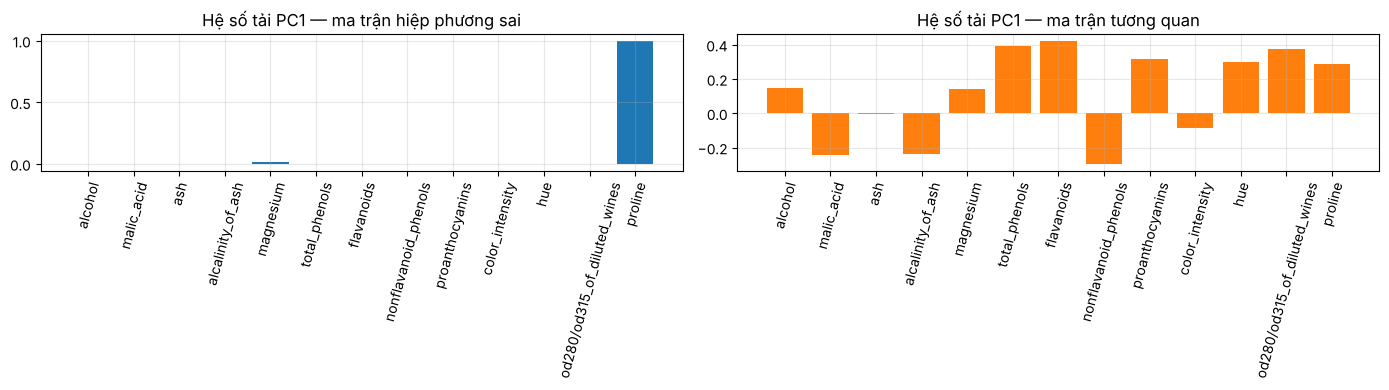
\includegraphics[width=0.95\linewidth]{img/C_c05_0.png}
\end{center}
\textbf{Kết luận:} PCA hiệp phương sai bị biến có số đo lớn nhất chi phối (proline có độ lệch chuẩn 315) và thay đổi hoàn toàn khi đổi đơn vị; PCA tương quan bất biến. Dùng tương quan khi các biến khác đơn vị — như đặc trưng rung ở Phần D.

\subsection{C.3 Kiểm chứng bổ đề Johnson–Lindenstrauss}
\begin{minted}{python}
def pairwise_sq_dists(Y):
    sq = (Y.astype(np.float64)**2).sum(1)
    G = Y.astype(np.float64) @ Y.T.astype(np.float64)
    D = sq[:, None] + sq[None, :] - 2 * G
    iu = np.triu_indices(len(Y), 1)
    return D[iu]
\end{minted}
\begin{itemize}
\item Bình phương khoảng cách mọi cặp bằng ma trận Gram ($\|x_i-x_j\|^2=\|x_i\|^2+\|x_j\|^2-2x_i^\top x_j$); \code{triu\_indices(n, 1)} lấy tam giác trên, bỏ đường chéo $\Rightarrow$ đúng $\binom{1000}2=499\,500$ cặp.
\item Dữ liệu và ma trận chiếu lưu \code{float32} để tiết kiệm bộ nhớ (ma trận $1000\times10\,000$), nhưng khoảng cách tính lại bằng \code{float64} để tránh mất chính xác khi trừ.
\item Phép chiếu: \code{Y = X\_jl @ R.T / np.sqrt(k)}; tỉ số méo \code{rho = pairwise\_sq\_dists(Y) / D\_orig}.
\end{itemize}
\begin{center}
\small
\begin{tabular}{rcccc}
\toprule
$k$ & $\max|\rho-1|$ & tỉ lệ cặp trong $1\pm0{,}1$ & trong $1\pm0{,}2$ & trong $1\pm0{,}3$ \\
\midrule
25 & $1{,}88\pm0{,}10$ & $0{,}274$ & $0{,}520$ & $0{,}717$ \\
100 & $0{,}82\pm0{,}08$ & $0{,}524$ & $0{,}848$ & $0{,}968$ \\
500 & $0{,}320\pm0{,}010$ & $0{,}885$ & $0{,}998$ & $1{,}000$ \\
1000 & $0{,}226\pm0{,}016$ & $0{,}974$ & $>0{,}9999$ & $1{,}000$ \\
2000 & $0{,}154\pm0{,}006$ & $0{,}9985$ & $1{,}000$ & $1{,}000$ \\
\bottomrule
\end{tabular}
\end{center}
Cận của bổ đề với $n=1000$: $k\ge5921$ ($\varepsilon=0{,}1$), $1595$ ($\varepsilon=0{,}2$), $768$ ($\varepsilon=0{,}3$). Ở $k=2000>1595$ mọi cặp đều trong $1\pm0{,}2$ ở cả 5 lần chạy; ở $k=1000>768$ mọi cặp trong $1\pm0{,}3$ — xác suất thành công thực tế gần 1, lớn hơn rất nhiều so với $1/n$.
\begin{center}
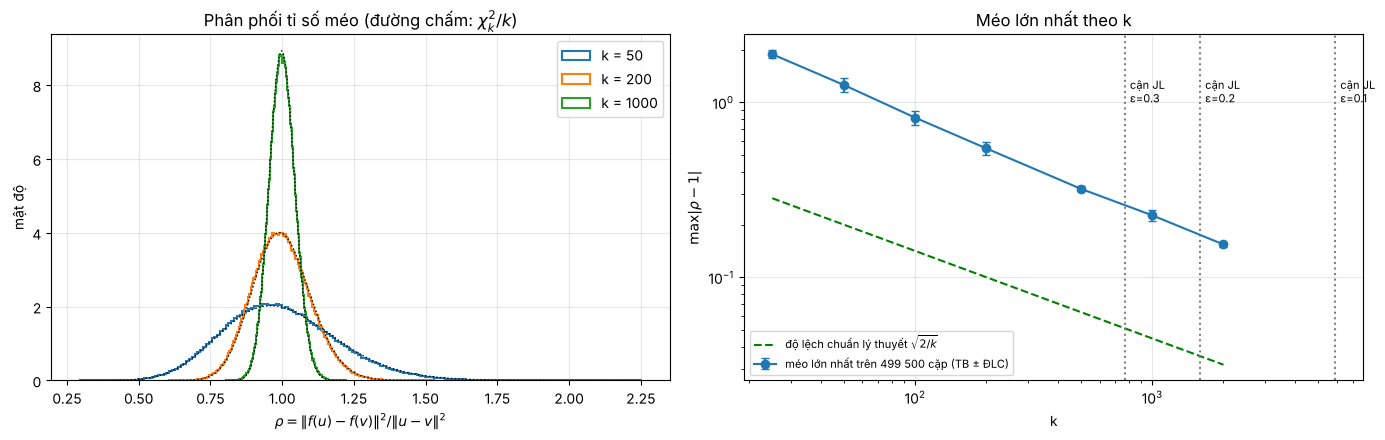
\includegraphics[width=\linewidth]{img/C_c08_0.png}
\end{center}
\textbf{Đọc hình:} trái — phân phối $\rho$ khớp $\chi^2_k/k$ (đường chấm), hẹp dần theo $1/\sqrt k$; phải — méo lớn nhất giảm theo $k$ với cùng độ dốc như $\sqrt{2/k}$.

\subsection{C.4 SVD đầy đủ, SVD ngẫu nhiên và lặp lũy thừa}
\begin{minted}{python}
def block_power_svd(A, k, max_iter=200, tol=1e-6, rng=None):
    rng = np.random.default_rng(rng)
    Q, _ = np.linalg.qr(A @ rng.standard_normal((A.shape[1], k)))
    s_old = np.zeros(k)
    for it in range(max_iter):
        Z, _ = np.linalg.qr(A.T @ Q)              # trực chuẩn hóa ở cả hai phía để ổn định
        Q, Rq = np.linalg.qr(A @ Z)               # Rq = Q^T A Z (k x k)
        s = np.linalg.svd(Rq, compute_uv=False)   # ước lượng rẻ các sigma để kiểm tra hội tụ
        if np.max(np.abs(s - s_old) / s) < tol:
            break
        s_old = s
    Ub, s, Vt = np.linalg.svd(Q.T @ A, full_matrices=False)
    return Q @ Ub, s, Vt, it + 1
\end{minted}
\begin{itemize}
\item Đây là lặp lũy thừa B.5 áp dụng cho cả khối $k$ vector (lặp trực giao): thay chuẩn hóa vector bằng QR. Tốc độ hội tụ theo $(\sigma_{k+1}/\sigma_k)^2$ mỗi vòng.
\item Khác SVD ngẫu nhiên: chỉ dùng $k$ cột (không có $p$) và lặp đến hội tụ thay vì cố định $q$ vòng.
\item \code{residual\_spectral\_norm}: ước lượng $\|A-USV^\top\|_2$ bằng 50 vòng lặp lũy thừa trên toán tử $x\mapsto(A-USV^\top)x$ mà \emph{không} tạo ma trận phần dư $10^4\times10^3$.
\item Sai số Frobenius dùng $\|A-\hat A_k\|_F^2=\|A\|_F^2-\sum\hat\sigma_i^2$ (đúng vì $\hat A_k=\hat U\hat U^\top A$ là phép chiếu).
\end{itemize}

\begin{center}
\small
\begin{tabular}{llccc}
\toprule
\textbf{Phổ} & \textbf{Phương pháp} & \textbf{Thời gian (s)} & $\|A-\hat A_k\|_2/\sigma_{k+1}$ & \textbf{max sai số $\hat\sigma_i$} \\
\midrule
nhanh & SVD đầy đủ & $2{,}14\pm0{,}14$ & $1{,}0000$ & $2\times10^{-15}$ \\
$e^{-(i-1)/10}$ & ngẫu nhiên $q=0$ & $0{,}06\pm0{,}01$ & $1{,}19\pm0{,}08$ & $5{,}8\times10^{-2}$ \\
& ngẫu nhiên $q=1$ & $0{,}12\pm0{,}01$ & $1{,}0000$ & $5{,}8\times10^{-4}$ \\
& ngẫu nhiên $q=2$ & $0{,}20\pm0{,}02$ & $1{,}0000$ & $6{,}2\times10^{-6}$ \\
& lặp lũy thừa khối (36 vòng) & $1{,}83\pm0{,}42$ & $1{,}0000$ & $1{,}3\times10^{-6}$ \\
\midrule
chậm & SVD đầy đủ & $2{,}21\pm0{,}08$ & $1{,}0000$ & $6\times10^{-16}$ \\
$i^{-1/2}$ & ngẫu nhiên $q=0$ & $0{,}06\pm0{,}01$ & $2{,}13\pm0{,}23$ & $0{,}44$ \\
& ngẫu nhiên $q=1$ & $0{,}13\pm0{,}03$ & $1{,}09\pm0{,}03$ & $0{,}087$ \\
& ngẫu nhiên $q=2$ & $0{,}21\pm0{,}05$ & $1{,}015\pm0{,}004$ & $0{,}032$ \\
& lặp lũy thừa khối (116 vòng) & $5{,}73\pm1{,}76$ & $1{,}0000$ & $8{,}9\times10^{-6}$ \\
\bottomrule
\end{tabular}
\end{center}
\begin{center}
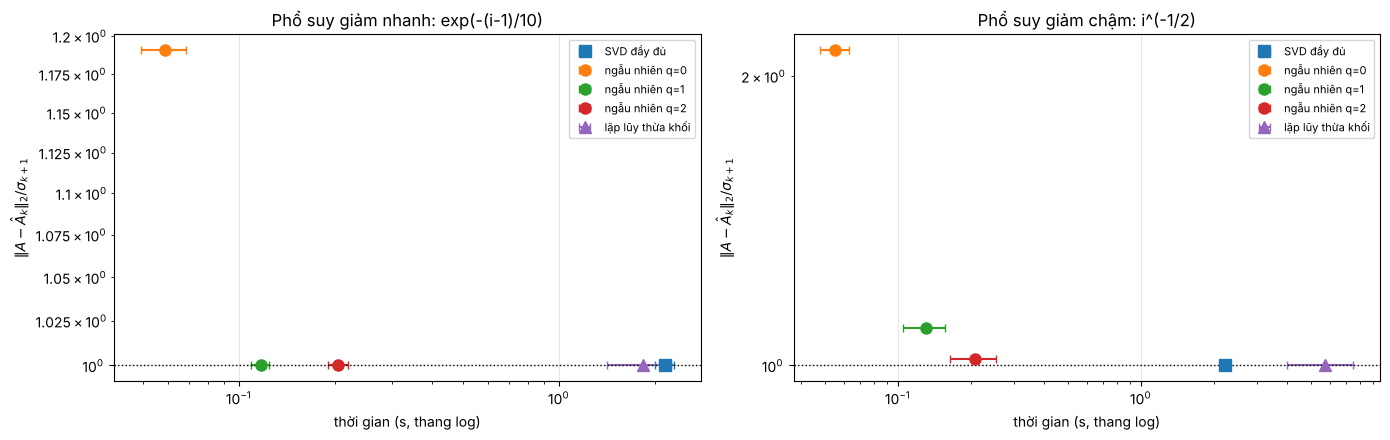
\includegraphics[width=\linewidth]{img/C_c12_0.png}
\end{center}
\textbf{Đọc kết quả:}
\begin{itemize}
\item SVD đầy đủ luôn tối ưu nhưng chậm (tính cả 1000 thành phần dù chỉ cần 20).
\item SVD ngẫu nhiên nhanh hơn 10–40 lần. Phổ giảm nhanh: $q=1$ đã tối ưu. Phổ giảm chậm: $q=0$ sai gấp 2 lần, các $\hat\sigma_i$ sai tới 44\%; cần $q=2$.
\item Lặp lũy thừa khối: 36 vòng khi $(\sigma_{21}/\sigma_{20})^2=e^{-0{,}2}\approx0{,}82$, nhưng 116 vòng khi tỉ số $=20/21\approx0{,}95$ — đúng như B.5 dự đoán; chậm hơn cả SVD đầy đủ trong trường hợp này.
\end{itemize}
\begin{ask}
\textbf{Nên chọn thuật toán nào cho Phần D?} Ma trận đặc trưng rung (vài nghìn cửa sổ $\times$ 45 đặc trưng) nhỏ nên SVD đầy đủ là đủ; SVD ngẫu nhiên hữu ích khi dùng phổ thô hàng nghìn chiều.
\end{ask}

%=====================================================================
\section{Bảng tra cú pháp dùng trong 3 notebook}
%=====================================================================
\begin{center}
\renewcommand{\arraystretch}{1.15}
\begin{tabularx}{\linewidth}{@{}>{\ttfamily\raggedright}p{6.2cm}X@{}}
\toprule
\normalfont\textbf{Cú pháp} & \textbf{Ý nghĩa} \\
\midrule
np.linalg.svd(A, full\_matrices=False) & SVD gọn; trả về \code{U}, \code{S} (vector), \code{Vt} $=V^\top$ \\
np.linalg.svd(A, compute\_uv=False) & chỉ các giá trị kỳ dị \\
np.linalg.eigh(C) / eigvalsh(C) & trị riêng (và vector riêng) ma trận đối xứng, \emph{tăng dần} \\
np.linalg.qr(Y) & trực chuẩn hóa các cột \\
np.linalg.norm(M, "fro") / (M, 2) & chuẩn Frobenius / chuẩn phổ \\
np.linalg.lstsq(P, A) & bình phương tối thiểu (dùng ở B.2) \\
X.mean(axis=0), X.std(axis=0, ddof=1) & trung bình / độ lệch chuẩn mẫu theo cột \\
U * S, S[:, None] * Vt & nhân cột / hàng với $\sigma_i$ (broadcasting) \\
np.argsort(x)[::-1] & chỉ số sắp giảm dần \\
np.searchsorted(cum, t) & vị trí đầu tiên trong mảng tăng có giá trị $\ge t$ \\
np.triu\_indices(n, 1) & chỉ số tam giác trên không gồm đường chéo \\
np.random.default\_rng(seed) & bộ sinh số ngẫu nhiên có hạt giống \\
scipy.linalg.subspace\_angles(A, B) & các góc chính giữa hai không gian con \\
stats.chi2.ppf, stats.f.ppf, stats.norm.ppf & phân vị của các phân phối $\chi^2$, $F$, chuẩn \\
stats.kstest(x, "chi2", args=(k,)) & kiểm định Kolmogorov--Smirnov \\
\bottomrule
\end{tabularx}
\end{center}

%=====================================================================
\section{Chuyển sang báo cáo LaTeX 25–40 trang}
%=====================================================================
\begin{center}
\renewcommand{\arraystretch}{1.2}
\begin{tabularx}{\linewidth}{@{}l>{\raggedright}p{7cm}X@{}}
\toprule
\textbf{Chương} & \textbf{Nội dung, nguồn} & \textbf{Số trang gợi ý} \\
\midrule
1. Giới thiệu & bài toán, đóng góp, cấu trúc & 1–2 \\
2. Cơ sở lý thuyết & SVD, PCA, ký hiệu; Mục 2 tài liệu này & 2–3 \\
3. Phần A & mỗi mục A.1–A.4: thuật toán (giả mã), cài đặt, thí nghiệm, bảng/hình ở Mục 2 & 6–8 \\
4. Phần B & 6 chứng minh — \code{b\_intro.tex}, \code{b\_B1.tex}…\code{b\_B6.tex} gửi kèm, \code{\textbackslash input} trực tiếp & 7–9 \\
5. Phần C & C.1 (\code{c\_C1.tex}), C.2–C.4 bảng và hình ở Mục 4 & 4–5 \\
6. Phần D & thí nghiệm, dữ liệu, mô hình, đánh giá, CWRU & 7–10 \\
7. Kết luận & tóm tắt, hạn chế, hướng phát triển & 1 \\
Phụ lục & thẻ dữ liệu, thẻ mô hình, khai báo sử dụng công cụ AI & 2–3 \\
\bottomrule
\end{tabularx}
\end{center}
Các file \code{.tex} gửi kèm dùng gói \code{amsmath}, \code{amssymb}; hình lấy từ thư mục \code{img/}. Đề yêu cầu khai báo phạm vi sử dụng công cụ AI tạo sinh trong phụ lục, và hội đồng có thể hỏi từng thành viên về bất kỳ chứng minh hay đoạn mã nào — mỗi người nên tự trình bày lại được ít nhất các chứng minh B.1, B.2 và giải thích \code{PCAMonitor}.

%=====================================================================
\section{Câu hỏi vấn đáp tổng hợp}
%=====================================================================
\renewcommand{\arraystretch}{1.3}
\begin{longtable}{@{}>{\raggedright\bfseries}p{5.4cm}p{10.2cm}@{}}
\toprule
Câu hỏi & Trả lời ngắn \\
\midrule
\endhead
PCA liên hệ với SVD thế nào? & $X_c=USV^\top$ $\Rightarrow$ hướng chính là cột của $V$, $\lambda_i=\sigma_i^2/(n-1)$, tọa độ $T=US$. \\
Vì sao SVD ổn định hơn trị riêng? & $\kappa(X^\top X)=\kappa(X)^2$; thí nghiệm A.1 cho thấy sai số $\varepsilon\kappa^2$ vs $\varepsilon\kappa$. \\
Ky Fan nói gì? & $\max_{U^\top U=I_k}\operatorname{tr}(U^\top\Sigma U)=\sum_{i\le k}\lambda_i$, đạt tại $k$ vector riêng đầu. \\
Eckart--Young chứng minh thế nào? & Cố định không gian cột $\to$ phép chiếu tối ưu (Pythagoras) $\to$ dùng Ky Fan cho $AA^\top$. \\
Tự mã hóa tuyến tính học được gì? & Đúng không gian con PCA; $DE=V_kV_k^\top$; $D$, $E$ không duy nhất. \\
JL: vì sao $k$ không phụ thuộc $d$? & $\|Rz\|^2/\|z\|^2\sim\chi^2_k$ với mọi $z$; Chernoff + chặn hợp chỉ phụ thuộc $n$, $\varepsilon$. \\
Lặp lũy thừa hội tụ nhanh cỡ nào? & Hình học với tỉ số $|\lambda_2/\lambda_1|$; với khối $k$ là $(\sigma_{k+1}/\sigma_k)^2$. \\
$p$, $q$ trong SVD ngẫu nhiên? & $p$: cột dự phòng; $q$: số vòng lặp lũy thừa, cần khi phổ giảm chậm. \\
Vì sao $T^2\sim\chi^2_k$? & Tọa độ chính chuẩn hóa là $k$ biến $\mathcal N(0,1)$ độc lập (Gauss không tương quan $\Rightarrow$ độc lập). \\
$T^2$ và SPE khác nhau ở đâu? & $T^2$: lệch trong không gian con chính; SPE: phá vỡ tương quan. Bổ sung cho nhau (A.4). \\
Vì sao $c_\alpha$ cùng dấu $h_0$? & Khi $h_0<0$, $(Q/\theta_1)^{h_0}$ là hàm giảm nên đuôi trên của $Q$ ứng với đuôi dưới của biến chuẩn. \\
Hiệp phương sai hay tương quan? & Tương quan khi biến khác đơn vị (C.2); bất biến khi đổi đơn vị. \\
Kernel PCA khác PCA? & PCA trong không gian đặc trưng ngầm; nhân tuyến tính trùng PCA; RBF bắt cấu trúc phi tuyến, nhạy với $\gamma$. \\
PCA tăng dần chính xác không? & Chính xác khi giữ đủ $d$ thành phần; cắt cụt $k<d$ là xấp xỉ (sai lệch $\sim10^{-3}$ độ ở A.2). \\
\bottomrule
\end{longtable}

\end{document}
